\documentclass[oneside,numbers,spanish]{ezthesis}

\usepackage[utf8]{inputenc}
\usepackage{mathtools}
\usepackage{amsmath}
\usepackage{booktabs}
\usepackage{amssymb}
\usepackage{comment}
\usepackage{amstext}
% \usepackage{subfigure}
% \usepackage{amsthm}
% \usepackage{booktabs}
% \usepackage{color}
\usepackage{hyperref}
% \usepackage{float}
% \usepackage{pdfpages}
% \usepackage{todonotes}
\usepackage{caption}
\usepackage{subcaption}
\usepackage{graphicx}
% \usepackage{fullpage}
\usepackage{verbatim}
\usepackage[spanish]{babel}
% \usepackage{wrapfig}
\usepackage{url}
% \usepackage{hyperref}
\usepackage{algpseudocode}
\usepackage{listings}\usepackage{color}
\usepackage{textcomp}\definecolor{listinggray}{gray}{0.9}
\usepackage{enumerate}
% \usepackage[left=2cm,right=2cm,bottom=2.5cm,top=2.5cm]{geometry}

\definecolor{lbcolor}{rgb}{0.9,0.9,0.9}

\lstset{language=C++,
  basicstyle=\small\sffamily,
  columns=fullflexible,
  upquote=true,
  extendedchars=true,
  texcl=true,
  mathescape=true,
  showspaces=false
}

\hypersetup{
    colorlinks,
    linkcolor={red!50!black},
    citecolor={blue!50!black},
    urlcolor={blue!80!black}
}


%% # Opciones disponibles para el documento #
%%
%% Las opciones con un (*) son las opciones predeterminadas.
%%
%% Modo de compilar:
%%   draft            - borrador con marcas de fecha y sin im'agenes
%%   draftmarks       - borrador con marcas de fecha y con im'agenes
%%   final (*)        - version final de la tesis
%%
%% Tama'no de papel:
%%   letterpaper (*)  - tama'no carta (Am'erica)
%%   a4paper          - tama'no A4    (Europa)
%%
%% Formato de impresi'on:
%%   oneside          - hojas impresas por un solo lado
%%   twoside (*)      - hijas impresas por ambos lados
%%
%% Tama'no de letra:
%%   10pt, 11pt, o 12pt (*)
%%
%% Espaciado entre renglones:
%%   singlespace      - espacio sencillo
%%   onehalfspace (*) - espacio de 1.5
%%   doublespace      - a doble espacio
%%
%% Formato de las referencias bibliogr'aficas:
%%   numbers          - numeradas, p.e. [1]
%%   authoryear (*)   - por autor y a'no, p.e. (Newton, 1997)
%%
%% Opciones adicionales:
%%   spanish         - tesis escrita en espa'nol
%%
%% Desactivar opciones especiales:
%%   nobibtoc   - no incluir la bibiolgraf'ia en el 'Indice general
%%   nofancyhdr - no incluir "fancyhdr" para producir los encabezados
%%   nocolors   - no incluir "xcolor" para producir ligas con colores
%%   nographicx - no incluir "graphicx" para insertar gr'aficos
%%   nonatbib   - no incluir "natbib" para administrar la bibliograf'ia

%% Paquetes adicionales requeridos se pueden agregar tambi'en aqu'i.
%% Por ejemplo:
%\usepackage{subfig}
%\usepackage{multirow}

%% # Datos del documento #
%% Nota que los acentos se deben escribir: \'a, \'e, \'i, etc.
%% La letra n con tilde es: \~n.

\author{Juan Antonio Navarro P\'erez}
\title{Ejemplo de una Tesis}
\degree{Doctor en Ciencias}
\supervisor{Nombre de mi Asesor}
\institution{Universidad de Alg\'un Sitio}
\faculty{Escuela de Ingenier\'ia y Ciencias}
\department{Departamento de Sistemas Computacionales}

%% # M'argenes del documento #
%% 
%% Quitar el comentario en la siguiente linea para austar los m'argenes del
%% documento. Leer la documentaci'on de "geometry" para m'as informaci'on.

%\geometry{top=40mm,bottom=33mm,inner=40mm,outer=25mm}

%% El siguiente comando agrega ligas activas en el documento para las
%% referencias cruzadas y citas bibliogr'aficas. Tiene que ser *la 'ultima*
%% instrucci'on antes de \begin{document}.
% \hyperlinking
\begin{document}

%% En esta secci'on se describe la estructura del documento de la tesis.
%% Consulta los reglamentos de tu universidad para determinar el orden
%% y la cantidad de secciones que debes de incluir.

%% # Portada de la tesis #
%% Mirar el archivo "titlepage.tex" para los detalles.

% %% ## Construye tu propia portada ##
%% 
%% Una portada se conforma por una secuencia de "Blocks" que incluyen
%% piezas individuales de informaci'on. Un "Block" puede incluir, por
%% ejemplo, el t'itulo del documento, una im'agen (logotipo de la universidad),
%% el nombre del autor, nombre del supervisor, u cualquier otra pieza de
%% informaci'on.
%%
%% Cada "Block" aparece centrado horizontalmente en la p'agina y,
%% verticalmente, todos los "Blocks" se distruyen de manera uniforme 
%% a lo largo de p'agina.
%%
%% Nota tambi'en que, dentro de un mismo "Block" se pueden cortar
%% lineas usando el comando \\
%%
%% El tama'no del texto dentro de un "Block" se puede modificar usando uno de
%% los comandos:
%%   \small      \LARGE
%%   \large      \huge
%%   \Large      \Huge
%%
%% Y el tipo de letra se puede modificar usando:
%%   \bfseries - negritas
%%   \itshape  - it'alicas
%%   \scshape  - small caps
%%   \slshape  - slanted
%%   \sffamily - sans serif
%%
%% Para producir plantillas generales, la informaci'on que ha sido inclu'ida
%% en el archivo principal "tesis.tex" se puede accesar aqu'i usando:
%%   \insertauthor
%%   \inserttitle
%%   \insertsupervisor
%%   \insertinstitution
%%   \insertdegree
%%   \insertfaculty
%%   \insertdepartment
%%   \insertsubmitdate

\begin{titlepage}
  \TitleBlock{\scshape\insertinstitution}
  \TitleBlock[\bigskip]{\scshape\insertfaculty}
  \TitleBlock{\Huge\scshape\inserttitle}
  \TitleBlock{\scshape
    Tesis presentada por \insertauthor \\
    para obtener el grado de \insertdegree}
  \TitleBlock{\insertsubmitdate}
  \TitleBlock[\bigskip]{\insertdepartment}
\end{titlepage}

%% Nota 1:
%% Se puede agregar un escudo o logotipo en un "Block" como:
%%   \TitleBlock{\includegraphics[height=4cm]{escudo_uni}}
%% y teniendo un archivo "escudo_uni.pdf", "escudo_uni.png" o "escudo_uni.jpg"
%% en alg'un lugar donde LaTeX lo pueda encontrar.

%% Nota 2:
%% Normalmente, el espacio entre "Blocks" se extiende de modo que el
%% contenido se reparte uniformemente sobre toda la p'agina. Este
%% comportamiento se puede modificar para mantener fijo, por ejemplo, el
%% espacio entre un par de "Blocks". Escribiendo:
%%   \TitleBlock{Bloque 1}
%%   \TitleBlock[\bigskip]{Bloque2}
%% se deja un espacio "grande" y de tama~no fijo entre el bloque 1 y 2.
%% Adem'as de \bigskip est'an tambi'en \smallskip y \medskip. Si necesitas
%% aun m'as control puedes usar tambi'en, por ejemplo, \vspace*{2cm}.




%% # Prefacios #
%% Por cada prefacio (p.e. agradecimientos, resumen, etc.) crear
%% un nuevo archivo e incluirlo aqu'i.
%% Para m'as detalles y un ejemplo mirar el archivo "gracias.tex".
%% Las secciones del "prefacio" inician con el comando \prefacesection{T'itulo}
%% Este tipo de secciones *no* van numeradas, pero s'i aparecen en el 'indice.
%%
%% Si quieres agregar una secci'on que no vaya n'umerada y que *tampoco*
%% aparesca en el 'indice, usa entonces el comando \chapter*{T'itulo}
%%
%% Recuerda que aqu'i ya puedes escribir acentos como: 'a, 'e, 'i, etc.
%% La letra n con tilde es: 'n.

\prefacesection{Agradecimientos}

Este trabajo no habr'ia sido posible sin el apoyo y el est'imulo de mi colega
y amigo, Doctor Rudolf Fliesning,  bajo cuya supervisi'on escog'i este tema y
comenc'e la tesis. Sr. Quentin Travers, mi consejero en las etapas finales
del trabajo, tambi'en ha sido generosamente servicial, y me ha ayudado de
numerosos modos, incluyendo el resumen del contenido de los documentos que
no estaban disponibles para mi examen, y en particular por permitirme leer, 
en cuanto estuvieron  disponibles, las copias de los  recientes extractos de
los diarios de campa'na del Vigilante Rupert Giles y la actual Cazadora la
se'norita Buffy Summers, que se encontraron con William the Bloody en 1998, y
por facilitarme el pleno acceso  a los diarios de anteriores Vigilantes
relevantes a la carrera de William the Bloody.

Tambi'en me gustar'ia agradecerle al Consejo la concesi'on de Wyndham-Pryce
como Compa'nero, el cual me ha apoyado durante mis dos a'nos de investigaci'on,
y la concesi'on de dos subvenciones de viajes, una para estudiar documentos
en los Archivos de Vigilantes sellados en Munich, y otra para la
investigaci'on en campa'na en Praga. Me gustar'ia agradecer a Sr. Travers,
otra vez, por facilitarme  la acreditaci'on  de seguridad para el trabajo en
los Archivos de Munich, y al Doctor Fliesning por su apoyo colegial y ayuda
en ambos viajes de investigaci'on.

No puedo terminar sin agradecer a mi familia, en cuyo est'imulo constante y
amor he confiado a lo largo de mis a'nos en la Academia. Estoy agradecida
tambi'en a los ejemplos de mis  difuntos hermano, Desmond Chalmers, Vigilante
en Entrenamiento, y padre, Albert Chalmers, Vigilante. Su coraje resuelto
y convicci'on siempre me inspirar'an, y espero seguir, a mi propio y peque'no
modo, la noble misi'on por la que dieron sus vidas. Es a ellos a quien dedico
este trabajo.

%% Por si alguien tiene curiosidad, este "simp'atico" agradecimiento est'a
%% tomado de la "Tesis de Lydia Chalmers" basada en el universo del programa
%% de televisi'on Buffy, la Cazadora de Vampiros.
%% http://www.buffy-cazavampiros.com/Spiketesis/tesis.inicio.htm


%% # 'Indices y listas de contenido #
%% Quitar los comentarios en las lineas siguientes para obtener listas de
%% figuras y cuadros/tablas.
\tableofcontents
%\listoffigures
%\listoftables

%% # Cap'itulos #
%% Por cada cap'itulo hay que crear un nuevo archivo e incluirlo aqu'i.
%% Mirar el archivo "intro.tex" para un ejemplo y recomendaciones para
%% escribir.
% \include{intro}
%\include{capitulo1}
%\include{capitulo2}
%\include{capitulo3}
%\include{conclu}


\chapter{Introducción}
\section{Objetivos}



El principal objetivo de la tesis es obtener una implementación del método de dinámica molecular basada en GPU, que siga un modelo de interacción de Lennard-Jones (potencial de no-unión), 
y que resuelva el cálculo de las fuerzas utilizando valores tabulados en el sistema de memoria provisto por la arquitectura. 

La forma funcional que describe el potencial de Lennard-Jones permitiría obtener una buena aproximación del valor utilizando una tabla de resultados precalculados. 
Además, el sistema de memorias de la arquitectura, que ha evolucionado considerablemente desde su creación, permite recuperar de forma eficiente el valor asociado en un esquema de tablas. 
De esta forma, se espera que la modificación resulte en una mejora de la performance manteniendo la correctitud en los resultados de la simulación. 

Una parte central del trabajo, además de evaluar la performance de las implementaciones, consiste en determinar que esta aproximación provee resultados correctos en términos del modelo físico subyacente.

\section{Estructura de la tesis}

En las siguientes secciones de este capítulo se exponen los fundamentos teóricos necesarios para comprender el marco en el que se insertan los distintos cálculos que se necesitan resolver. 
Se detalla el método que se implementa y se exhibe una representaci\'o abstracta y generalizada del algoritmo.

En el capítulo 2, se analiza en detalle la arquitectura sobre la cual se trabaja. Se tienen en cuenta tanto las propiedades físicas del hardware como las del modelo de programación asociado,
poniendo \'enfasis en las caracter\'isticas que ser\'an utilizadas para este trabajo.
Finalmente, se presentan de manera concisa los distintos aspectos de performance que se deben tener en cuenta a la hora de trabajar sobre este tipo de procesadores.

Más adelante, en el capítulo 3, se exponen los algoritmos que se desarrollaron a partir de los trabajos existentes en la literatura, y las modificaciones planteadas con respecto a estos. 
Se explican, adem\'as, las propiedades de estos algoritmos que permiten obtener una implementación eficiente haciendo uso de arquitecturas altamente paralelas.

Luego, en el capítulo 4, se explica el funcionamiento del código desarrollado para el procesador gráfico, justificando las decisiones que se tomaron en cada caso y detallando 
cómo se tuvieron en cuenta los aspectos de performance previamente mencionados. 

Todos los resultados obtenidos, que incluyen la búsqueda de parámetros óptimos, análisis de performance de las implementaciines y de la calidad numérica de los cálculos realizados, se presentan en el capítulo 5.

Por último, en el capítulo número 6, se discute el alcance que tendrán los resultados obtenidos y el trabajo a futuro que deja esta tesis.


\section{El método de dinámica molecular}

\subsection{Fundamentos}


Los sistemas químicos de interés como las proteínas suelen ser complejos de estudiar debido a su gran tamaño. 
La superficie de energía libre, que describe la energía del sistema y a partir de la cual se podrían derivar todas 
las propiedades termodinámicas y cinéticas de interés, es una función 3N dimensional (siendo N el número de partículas del sistema), 
lo que hace imposible derivar analíticamente las propiedades por el altísimo costo computacional asociado.

Otra forma de analizar estos sistemas es mediante una aproximación numérica, a través de simulaciones computacionales.
La simulación computacional de biomoléculas involucra la exploración de su superficie de energía libre, la cual, debido a la complejidad de estos sistemas, es altamente accidentada, 
contiene una gran cantidad de mínimos locales y de barreras de energéticas. 
De esta forma, si los parámetros de la simulación están correctamente definidos, el conjunto de conformaciones adoptadas durante la ejecución será representativo del ensamble 
real de conformaciones posibles del sistema, lo que permite estimar las propiedades de interés.

Los métodos de simulación molecular nos permiten, entonces, obtener una serie de configuraciones representativas del sistema, de modo que las propiedades termodinámicas extraídas del mismo se correspondan 
de manera precisa con los valores reales.
Una de las formas de obtener estas configuraciones es mediante el método de dinámica molecular(DM). 
Este método implica simular la progresión temporal ``real'' del sistema, obteniendo distintas conformaciones a medida que avanza el tiempo de simulación.

La técnica de simulación de dinámica molecular se basa en resolver las ecuaciones de movimiento de Newton para cada átomo del sistema; así, en cada paso de la ejecución 
se calculan las fuerzas entre las partículas, derivandolas del potencial de interacción entre éstas.

Las ecuaciones de Newton relacionan las fuerzas resultantes del potencial con la aceleración que tendrá cada particula y, por lo tanto, el cambio en la velocidad y en la posición con el tiempo. 
Dado que el potencial(y su derivada) son funciones continuas dependiente de la posición, los cambios en las velocidades y posiciones resultan de una integración a lo largo de la trayectoria de la partícula.


\subsection{Esquema general del método}

En la práctica, la integración de las ecuaciones de Newton se calcula mediante el llamado Algoritmo de Verlet, el cual resuelve la integración con una ecuación discreta donde las posiciones estan separadas por intervalos de tiempo (``dt'') . 
Usando las fuerzas resultantes, junto con las posiciones y velocidades de las partículas correspondientes a la iteración, el algoritmo de Verlet calcula las nuevas posiciones y velocidades en un intervalo de tiempo posterior. 
De este modo se genera una trayectoria, determinada por las posiciones de las particulas en cada paso de la simulación. 
Esta trayectoria describe como cambia la conformación espacial del sistema a lo largo del tiempo. 
La elección del parámetro \textit{dt} es una situación de compromiso ya que un valor muy chico, si bien representa la propagación del movimiento de forma mas precisa(mas cercana al valor real de la integración), 
requiere una mayor cantidad de cálculos para alcanzar un mismo tiempo total de simulación. 



El esquema general del método se puede ver en la figura \ref{esquemaMD}.

% **********************************************************************
% ***************CAMBIAR LA FIGURA POR UNA SIMILAR EN ESPAÑOL **********
% **********************************************************************

\begin{figure}[!ht]
\begin{center}
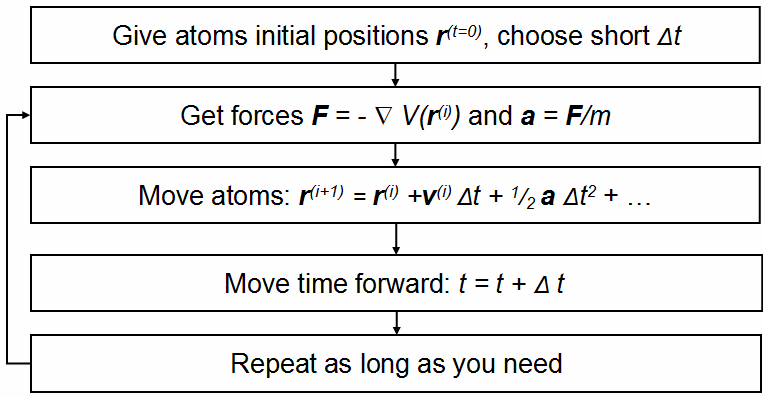
\includegraphics[keepaspectratio, width=0.5\textwidth]{img/md/mdalgorithm.png}
\end{center}
\caption{Esquema general del algoritmo de dinámica molecular}
\label{esquemaMD}
\end{figure}





% *********************
% ****QUE OTROS DATOS RELEVANTES OBTENGO DE LA SIMULACION??
%********************** 

  
El resultado de la simulación es, fundamentalmente, una trayectoria representada por las posiciones de cada una de las partículas a lo largo de un cierto tiempo.
No se va a detallar acerca del análisis posterior de este resultado pero es relevante decir que la longitud de trayectoria que podamos obtener en un tiempo de cómputo razonable es lo que limita el tipo de proceso químico que podremos estudiar.
Para poder estudiar un proceso de interés, entonces, es necesario que la simulación alcance la escala de tiempo en la cual éste ocurre. 
Un mayor tiempo de simulación equivale a realizar más pasos y por lo tanto más cálculos totales, aumentando así el tiempo de cómputo requerido.

Por su parte, simular sistemas más grandes (con mayor cantidad de partículas) implica un incremento en la cantidad de cálculos por cada paso y por lo tanto un mayor costo computacional. 
Además, la función que describe las propiedades del sistema tiene por naturaleza una mayor cantidad de variables, debido a esto es necesario correr la simulación durante más tiempo para poder llegar 
a un conjunto de conformaciones que sea representativo del ensamble real.




\subsection{La función potencial}


En la utilización del método de dinámica molecular, el potencial(V) que permite derivar las fuerzas entre partículas se obtiene modelando al sistema molecular a través de la mecánica clásica (método conocido como mecánica molecular o MM).
Usando un método de MM, se ignoran los electrones y la naturaleza cuántica de estos. La energía potencial del sistema, entonces, depende exclusivamente de las posiciones de los núcleos atómicos. 
Se modela cada molécula como un conjunto de sitios -que representan los átomos que la componen- y resortes -que representan los enlaces químicos entre estos- junto con un potencial parametrizado \textit{ad hoc}.

Este potencial es una función matemática que depende exclusivamente de las posiciones de los átomos, la cual se ajusta a las interacciones observadas experimentalmente entre los componentes del sistema. 
Este tipo de repesentacion simplificada del sistema permite reducir la complejidad de los cálculos necesarios para la simulación y, por lo tanto, el costo computacional asociado. 
La desventaja de este tipo de modelos es que limita el conjunto de procesos que se pueden estudiar. 
Por ej. no es posible hacer análisis de reacciones quimicas que impliquen ruptura o formación de enlaces ya que estos no son considerados con suficiente detalle. 
Mas allá del método MM, existen otras formas de representar al sistema con mayor detalle y aproximaciones que utilizan esquemas híbridos de representación\cite{senn2009qm} buscando balancear el costo computacional y
el detalle que se obtiene del proceso estudiado.
En los ultimos años, surgieron también modelos de representación menos detallados, conocidos como de grano grueso(coarse-grained)\cite{noid2013perspective}, apuntando principalmente a simular sistemas biológicos, que se caracterizan por poseer una gran cantidad de átomos.

Las interacciones representadas en el método de MM se pueden agrupar en dos tipos:

\begin{description}
 \item [De unión:] Describen las interacciones entre dos átomos unidos entre si directamente o hasta dos enlaces de distancia. 
 Consisten en aquellos términos del potencial cuya energía se ve afectada por los estiramientos de los enlaces, las flexiones de los ángulos entre dos átomos, y la rotación de dos átomos adyacentes sobre un eje (ángulos dihedros). Los estiramientos y las flexiones angulares son modeladas mediante un oscilador armónico, mientras que las rotaciones de los enlaces en el plano son modeladas mediante una función trigonométrica.

\item [De no unión:] describen la interacción entre átomos ubicados a más de 3 enlaces de distancia de la misma molécula, o bien entre átomos de moléculas distintas, y consisten en un término para la
contribución electrostática calculada mediante la Ley de Coulomb, y un término para la contribución de Van Der Waals modelada por un potencial de Lennard-Jones 12-6.


\end{description}



El esquema general de la función potencial suele tomar una forma similar al representado en la figura \ref{potencialAmber} \\
% \includegraphics[]{img/ecPotencialAmber.png}
% \begin{figure}[h]
% \includegraphics[keepaspectratio, width=1.0\textwidth]{img/ecPotencialAmber.png}
% \caption{Ejemplo de potencial de interacción del paquete de software Amber}
% \label{Fig:Amber}
% \end{figure}
% \vspace{2pt}
\begin{figure}[!ht]
% \begin{center}
\includegraphics[keepaspectratio, width=\textwidth]{img/md/ecPotencialAmber.png}
% \end{center}
\caption{Ejemplo de potencial de interacción del paquete de software Amber}
% \caption{Esquema general del algoritmo de dinámica molecular}
\label{potencialAmber}
\end{figure}

En azul se representan los términos matemáticos que modelan las interacciones de unión (1. Término de estiramiento de enlaces; 2. Término de flexión angular; 3. Término de rotación de ángulos diedros), y en rojo
las interacciones de no unión (Potencial de Lennard-Jones 12-6 e interacción Coulómbica).

Los parámetros que se observan en esta función potencial (las constantes $K_b, K_{\theta}$ y $V_n$ , los valores de equilibrio $b_0$, $\theta_0$ y $\delta$ , 
las constantes A y B correspondientes al potencial Lennard-Jones, y las cargas q) deben ser ajustados especialmente para cada molécula individual que se desee incluir en la 
simulación. Estos parámetros se suelen obtener tanto de datos experimentales, como así también de rigurosos cálculos cuánticos, y en ocasiones emplean correcciones empíricas.
Al conjunto o "set" de parámetros derivados para utilizarse de forma conjunta en una simulación se lo conoce como campo de fuerzas.

Esta parametrización del modelo de interacciones representa la principal diferencia entre los distintos paquetes de software para simulaciones de dinámica molecular. 
Las distintas versiones suelen tener uno o mas campos de fuerzas propios para utilizar en las simulaciones. 
Estos campos de fuerzas estan parametrizado específicamente para el tipo de sistema que se intenta simular, logrando que se ajuste lo mejor posible a la realidad.
De esta forma, existen versiones específicas para simular distintos sistemas biologicos (proteínas, ácidos nucleicos), otros que intentan abarcar a sistemas de química orgánica en general, etc.
La eleccion del campo de fuerzas es un aspecto importante de la simulacion de DM ya que éste define como se relacionan distintas partes de una misma molécula, como cada átomo se ve afectado por el entorno y como las condiciones contribuyen a la estructura molecular. 

Para estudiar procesos moleculares de interés mediante la técnica de dinámica molecular, es necesario alcanzar la escala correcta de tiempo en la cual ocurre este procesos y, a la vez, asegurarse que el modelado físico
que se está utilizando sea adecuado, de manera que los resultados obtenidos sean precisos.\cite{piana2014assessing}



\subsubsection{Potencial de Lennard-Jones}

El cálculo de las interacciones de no unión es un paso importante en el algoritmo ya que implica la mayor parte del costo computacional asociado a la simulación. 
Esto se debe a que es necesario calcularlo entre todos los elementos del sistema. 
En particular, es importante el término correspondiente al potencial de Lennard-Jones porque este existe siempre, independientemente de la carga neta en las partículas que interaccionan.

La expresión mas común que representa este potencial es: 
\begingroup
\fontsize{14pt}{5pt}
\begin{equation}\label{lennardEquation} V_{LJ}(r)= 4 \epsilon [ (\sigma/r)^{12} - (\sigma/r)^6] \end{equation}
\endgroup
Esta ecuación está compuesta por dos términos representando fuerzas opuestas:
El primer término ($(\sigma/r)^{12}$) representa fuerzas de repulsión que actúan a corta distancia.
El segundo término ($(\sigma/r)^{6}$) representa fuerzas de atracción que actúan en un rango mayor de distancias.

% \vspace{10pt}
Es usual reagrupar los términos $\sigma$ y  $\epsilon$ usando  
$A=4\epsilon\sigma^{12}  $  y  $B=4\epsilon\sigma^6$ para obtener una forma simplificada de la ecuación:   \begin{equation}  V_{LJ}(r)= [ (A/r^{12}) - (B/r^6)] \end{equation}

% \vspace{20pt}


En la figura \ref{lennardimage} se puede ver el comportamiento físico que describe este modelo de interacción:

% ***BUSCAR UNO QUE ESTE ASI DETALLADO PERO EN CASTELLANO****

% \vspace{14pt}
% \begin{center}
% \end{center}

\begin{figure}[!ht]
\centering
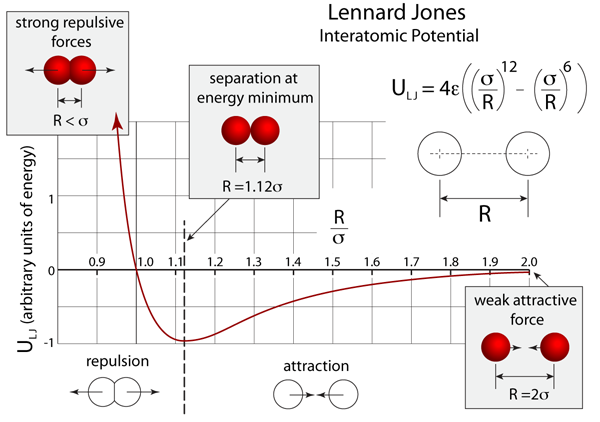
\includegraphics[height=8cm,keepaspectratio, width=\textwidth]{img/md/LennardJonesFull.png}
% \includegraphics[keepaspectratio, height=10cm ,width=0.5\textwidth]{img/minimage.png}
\caption{Comportamiento del potencial de Lennard-Jones}
\label{lennardimage}
\end{figure}

Se pueden observar dos regiones separadas que representan las fuerzas opuestas de la ecuación. 
Estos segmentos están separados por un valor mínimo que se corresponde con el equilibrio entre el componente repulsivo y el de atracción. 
La distancia de equilibrio (que toma un valor de $2^{1/6}\approx1.12$) se obtiene derivando el potencial e igualándolo a 0.

En el primer segmento de la curva ($r<1.12\sigma$), el valor del potencial esta gobernado por el componente repulsivo. 
Este valor aumenta exponencialmente al disminuir la distancia, toma un valor $V=0$ cuando $r=\sigma$, y se hace positivo para valores de $r<\sigma$ indicando una fuerza repulsiva entre los átomos.

En el punto de equilibrio ($r=1.12\sigma$) el potencial toma el valor mínimo $V=-\epsilon$.

En el segundo segmento de la curva ($r>1.12\sigma$), el valor del potencial esta gobernado por el componente atractivo. El valor del potencial (siempre negativo, indicando una fuerza de atracción) se acerca a 0 a medida que la distancia se acerca a infinito. 


A partir de la forma que toma el potencial de L-J resulta razonable pensar que, si se desprecia el aporte de este potencial para interacciones entre partículas a una distancia mayor que cierto valor de corte, 
se podrá obtener una buena aproximación del comportamiento a la vez que se reduce considerablemente la cantidad de cálculos necesarios en cada paso de la simulación.
Esta es una aproximación que proveen varias de las versiones implementadas del método, permitiendo que el usuario defina un valor de corte(\textit{cutoff}). 
En cada paso, si dos partículas están separadas por una distancia mayor que el \textit{cutoff} se les asigna automáticamente un valor de potencial $V_{LJ}=0$ asumiendo que se está realizando una buena aproximación, 
lo que elimina el costo de tener que calcular el valor real. 
Depende del usuario definir un \textit{cutoff} que sea coherente con el sistema y simulación a realizar.

Como se mencionó previamente, el potencial de L-J ofrece una aproximación generalmente buena de las interacciones de no unión en modelos moleculares y, dada su simplicidad, es incluido en gran parte de los campos de fuerzas utilizados en dinámica molecular.
Es por esto que la optimización del calculo asociado tendría un gran impacto en este métdodo de simulación. 
Además, la forma funcional implica que existe, al menos débilmente, entre todos los pares de particulas del sistema, lo que se traduce en una gran cantidad de cálculos por paso. 
El cálculo de este potencial representa así la mayor parte del costo computacional asociado a la simulación. 


\subsection{Condiciones de frontera} \label{frontera}

Hasta aquí hemos definido al sistema como el conjunto de átomos sobre los cuales realizamos la simulación. 
Sin embargo, los sistemas reales tienen, en términos prácticos, un tamaño infinito. 
Es decir, independientemente de cuántos elementos podamos incluir en nuestro conjunto de simulación, el número de parículas(N) será siempre despreciable con respecto al número de componentes del sistema macroscópico real.

Si no se implementa ninguna condición particular a los límites de nuestro sistema, se estaría simulando un conjunto de partículas en el vacío. 
De esta forma, las interacciones ocurrirían solo entre las particulas del conjunto de simulación que definimos, sin tener en cuenta ningún elemento en el contexto.
Además, no habría limites definidos para las posibles posiciones de las partículas, las cuales pueden, por lo tanto, difundir libremente durante la ejecución.

Este tipo de simulaciones raramente es útil ya que no representan situaciones realistas. Se debe tener en cuenta, entonces, condiciones especiales que tendrán los limites en la simulación para que estos representen de forma adecuada a los sistemas de interés.
Existen distintas aproximaciones para implementar estas condiciones en los límites manteniendo un conjunto reducido de partículas.

Utilizar condiciones periódicas de borde es la forma mas común de simular un sistema infinito. Aplicando esta condición, las partículas están contenidas en una caja de simulación con un tamaño definido. 
Esta caja es replicada virtualmente al infinito en las tres direcciones del eje cartesiano, llenando completamente el espacio.
Todas las imágenes de las partículas se mueven de forma idéntica a la partícula central. De hecho, sólo una de ellas(la que se encuentra en la caja central) es la que efectivamente se está simulando.
Cuando una partícula entra o sale de la caja central, una imagen de ella entra o sale por la cara opuesta de esta región, de manera tal que el número de partículas contenidas en la región de simulación siempre se conserva.
Se puede ver que, de esta forma, los límites del sistema que se está simulando son virtualmente eliminados y no tienen ningún efecto sobre la simulación.
Como resultado de esto, cada partícula perteneciente al conjunto de simulación interactúa no solo con las demás partículas de este, sino también con las imágenes virtuales que estamos teniendo en cuenta.

Al parecer, el número de interacciones (y por lo tanto la cantidad de cálculos a realizar) se incrementará enormemente con esta nueva condición. 
Sin embargo, esto puede evitarse si se utiliza un potencial con un rango finito, dado que en este caso se pueden ignorar las interacciones entre partículas separadas por una distancia mayor a cierto valor de \textit{cutoff}.
En este caso, teniendo un valor de cutoff $R_{c}$ y definiendo una caja de simulación cuyo lado menor tenga una longitud $L_m$: 
Si hacemos cumplir que $L_m>2R_{c}$, entonces se verá que, como máximo, solo una de las imágenes de cada particula quedará dentro del rango del cutoff y por lo tanto deberá ser considerada.
Este método, conocido como el criterio de imagen mínima, permite limitar el número de cálculos necesarios considerando solo la imagen mas cercana e ignorando el resto. 
De esta forma se puede cumplir con las características infinitas del sistema real y las propiedades impuestas por el potencial, logrando una mejor aproximación en la simulación.
La figura \ref{minimage} muestra una representación gráfica de este método. 


\begin{figure}[!ht]
\centering
\includegraphics[keepaspectratio, height=10cm ,width=0.5\textwidth]{img/md/minimage.png}
\caption{Criterio de imagen mínima para condiciones periódicas de frontera. Los círculos sin relleno representan todas las imágenes de la misma particula i}
\label{minimage}
\end{figure}


% propiedades fisicas van a depender del tamano de la caja
% Agregar detalles de sumatoria de Ewald ?










\subsection{Estado del arte}



Desde que fue desarrollado, el método ha sido de una gran utilidad y ha demostrado una posiblidad de aplicación a futuro mucho mayor. 
Esta posiblidad de aplicarlo a sistemas cada vez mas grandes y procesos en escalas de tiempo mayores es lo que impulsó una constante búsqueda de mejoras sobre el algoritmo inicial.
Se han desarrollado entonces una gran cantidad de estrategias que apuntan a optimizar el costo computacional asociado al método, sin sufrir una pérdida considerable en la precisión.

Para sistemas típicos de biomoleculas en donde el sistema está compuesto por una macromolécula(ej. proteínas) rodeada de un solvente líquido, es posible utilizar una aproximación conocida 
como solvente implícito\cite{tsui2000theory}.
En este modelo, el solvente se representa como un medio continuo alrededor del sistema central en lugar de representar explícitamente todas las unidades que lo componen, 
reduciendo considerablemente el número de cálculos necesarios para evaluar la interacción con las moléculas de solvente. Al ser una aproximación, tiene ciertas limitaciones en cuanto 
a la precisión y al tipo de sistemas en los que puede ser aplicado.

El calculo asociado al componente electroestático puede ser optimizado usando el método conocido como sumatoria Ewald \cite{toukmaji1996ewald}. 
Este método permite aproximar el cálculo de interacciones que actúan en un amplio rango de distancias sobre sistemas periódicos. 

Otra adaptación muy utilizada es la implementación de una lista de vecinos para cada partícula \cite{plimpton1995fast}. 
Esta lista mantiene las moleculas que estan dentro del rango de interacción(distancia menor al \textit{cutoff}) y son los únicos que se tendrán en cuenta a la hora de hacer el cálculo. 
La optimización se basa en que la lista solo se actualiza cuando se ejecuta una cierta cantidad de pasos definida como parámetro. 
Este valor se deriva experimentalmente a partir de simulaciones de prueba y es el parámetro que balancea la optimización y la precisión: cuanto mas se demora la actualizacién mejor es el 
tiempo de ejecución pero menos representativa es la lista acerca de la realidad del entorno y, por lo tanto, menos preciso es el cálculo.

Existe una gran cantidad de variantes del algoritmo, solo se han mencionado algunos de los caminos en los que se ha avanzado realizando modificaciones con respecto a la descripción inicial.

En cuanto a las arquitecturas de cómputo, las implementaciones sobre GPU, que son el centro de este trabajo, se han establecido como estándares para las implementaciones actuales del método \cite{stone2010gpu,friedrichs2009accelerating}.
Esto se debe al gran poder de cómputo que proveen en relación al costo económico, teniendo en cuenta que el algoritmo es altamente paralelizable y este tipo de hardware provee las condiciones
necesarias para una implementación eficiente.

% 
% Con este contexto , las capacidades de cálculo actuales permiten realizar simulaciones de dinámica molecular en sistemas de hasta XXX átomos aproximadamente, sobre un intervalo de tiempo del 
% orden de YYYYYYY  micro/pico/******segundos).

Si bien se ha avanzado mucho desde el desarrollo del método, existen múltiples procesos de interés que podrían ser abordados mediante experimentos de simulación computacional pero que el intervalo de 
tiempo en el cual ocurren no es posible de ser alcanzado con los recursos disponibles hoy en dia.
Esta situación hace que se destine una gran cantidad de esfuerzo para continuar las mejoras en el método y mantener las implementaciones a la par de las arquitecturas disponibles, 
las cuales han avanzado considerablemente teniendo en cuenta que hace un largo tiempo que el método comenzó a ser aplicado al estudio de proteinas \cite{mccamm0n1977dynamics}
El presente trabajo intenta, entonces, evaluar posibles modificaciones que permitan adecuar las implementaciones más actuales del método para explotar al máximo todas las características 
que ofrece la arquitectura de GPU. 

% ACA PODRIA PONER QUE LOS QUIMICOS TIENEN MUCHOS PROBLEMAS PARA PROBAR LAS COSAS Y BLA BLA BLA YA QUE TIENEN ADAPTACIONES MUY PUNTUALES DEL SISTEMA QUE EJECUTAN ) 
% ADEMAS TENDRIA QUE EXPLICAR EN ALGUN LADO QUE ESTA IMPLEMENTACION SE ENMARCA EN UN PROYECTO  DE MAYOR ESCALA QUE BUSCA IMPLEMENTAR UN ALGORITMO  COARSE-GRAINED
% DESDE CERO, Y  LOS ALGORITMOS COARSE GRAINED SE BASAN EN PROBAR POTENCIALES AD-HOC, A DIFERENCIA DE LOS METODOS MAS DE QM(QUE BUSCAN IR A UNA MENOR ESCALA)
% ENTONCES ES NECESARIO TENER UNA IMPLEMENTACION QUE PERMITA FACILMENTE MODIFICAR LA IMPLEMENTACION

% TAMBIEN PUEDO DECIR QUE UNA IDEA ES TRATAR DE ABSTRAER UN POCO EL PROBLEMA SUBYACENTE Y PLANTEAR LOS COMPONENTES DEL ALGORITMO Y LA FORMA EN QUE ESTOS PUEDEN EVOLUCIONAR HACIA MEJORES PERFORMANCES(YA QUE ).  










\def\nvidia{Nvidia}
\def\lio{LIO}
\def\plotwidth{350px}
\def\plotwidthbigger{390px}
\def\plotwidthtres{210px}
\def\plotwidthsmaller{310px}
\def\plotwidthverysmall{240px}
\def\thread{\textit{thread}}
\def\threads{\textit{threads}}
\def\turboboost{\textit{Turbo Boost}}
\def\hyperthreading{\textit{Hyper-Threading}}
\def\speedup{\textit{speedup}}
\def\Speedup{\textit{Speedup}}
\def\performance{\textit{performance}}


% ESTE CAPITULO LO COPIO ENTERO DE OTRAS TESIS  ( SOLO AGREGO ALGUNOS DETALLES QUE USO EN LAS IMPLEMENTACIONES )

\chapter{La arquitectura GPU}

\section{Introducci\'on}

Este trabajo se centra en la arquitectura GPU desarrollada por \nvidia{}, conocida como CUDA por las siglas en ingles de \textit{Compute Unified Device Architecture}.
CUDA surge naturalmente de la aplicaci\'on del hardware desarrollado para problemas gr\'aficos, pero aplicados al c\'omputo cient\'ifico.

Las placas de v\'ideo aparecen en 1978 con la introducci\'on de Intel del chip \texttt{iSBX 275}.
En 1985, la Commodore Amiga inclu\'ia un coprocesador gr\'afico que pod\'ia ejecutar instrucciones independientemente del CPU, un paso importante en la separaci\'on y especializaci\'on de las tareas.
En la d\'ecada del 90, m\'ultiples avances surgieron en la aceleraci\'on 2D para dibujar las interfaces gr\'aficas de los sistemas operativos y, para mediados de la d\'ecada, muchos fabricantes estaban incursionando en las aceleradoras 3D como agregados a las placas gr\'aficas tradicionales 2D.
A principios de la d\'ecada del 2000, se agregaron los \textit{shaders} a las placas, peque\~nos programas independientes que corr\'ian nativo en el GPU, y se pod\'ian encadenar entre s\'i, uno por pixel en la pantalla~\cite{Mark2003}.
Este paralelismo es el desarrollo fundamental que llev\'o a las GPU a poder procesar operaciones gr\'aficas \'ordenes de magnitud m\'as r\'apido que el CPU.

En el 2006, \nvidia{} introduce la arquitectura G80, que es el primer GPU que deja de resolver \'unicamente problemas de gr\'aficos para pasar a un motor gen\'erico donde cuenta con un set de instrucciones consistente para todos los tipos de operaciones que realiza (geometr\'ia, vertex y pixel shaders)~\cite{cudaHandbook}.
Como subproducto de esto, la GPU pasa a tener procesadores sim\'etricos m\'as sencillos y f\'aciles de construir.
Esta arquitectura es la que se ha mantenido y mejorado en el tiempo, permitiendo a las GPU escalar masivamente en procesadores simples, de baja frecuencia de reloj y con una disipaci\'on t\'ermica manejable.

Los puntos fuertes de las GPU modernas consisten en poder atacar los problemas de paralelismo de manera pseudo-expl\'icita, y con esto poder escalar ``f\'acilmente'' si solamente se corre en una placa con m\'as procesadores~\cite{cudaProgrammingGuide}.

T\'ecnicamente, esta arquitectura cuenta con entre cientos y miles de procesadores especializados en c\'alculo de punto flotante, procesando cada uno un \textit{thread} distinto pero
trabajando de manera sincr\'onica agrupados en bloques.
Cada procesador, a su vez, cuenta con entre $63$ a $255$ registros~\cite{NvidiaFermi,NvidiaKepler}.
Las GPU cuentas con m\'ultiples niveles de cache y memorias especializadas (subproducto de su dise\~no fundamental para gr\'aficos).
Estos no poseen instrucciones SIMD, ya que su dise\~no primario esta basado en cambio, en SIMT (\textit{Single Instruction Multiple Thread}), las cuales se ejecutan en los bloques sincr\'onicos de procesadores.
De este modo, las placas modernas como la \nvidia{} Tesla K40 alcanzan poder de c\'omputo de $4.3$ TFLOPs (4300 mil millones de operaciones de punto flotante por segundo) en c\'alculos de precisi\'on simple, $1.7$ TFLOPs en precisi\'on doble y $288$ GB/seg de transferencia de memoria, usando $2880$ CUDA Cores~\cite{NvidiaKeplerDatasheet}.
Para poner en escala la concentraci\'on de poder de c\'alculo: una computadora usando solo dos de estas placas posee una capacidad
de c\'omputo comparable a la supercomputadora m\'as potente del mundo en Noviembre 2001~\cite{Top500November2001}.
Una comparativa del poder de c\'omputo te\'orico entre GPUs y CPUs puede ver en la figura~\ref{fig:cuda-gflops}.

\begin{figure}[htbp]
    \centering
    \includegraphics[width=\plotwidthsmaller]{img/arq/cuda-gflops_ES.pdf}
    \caption{Picos te\'oricos de \performance{} en GFLOPS/s. Tomado de~\cite{cudaProgrammingGuide}.}
    \label{fig:cuda-gflops}
\end{figure}

Para poder explotar la arquitectura CUDA, los programas deben ser dise\~nados de manera de que el problema se pueda particionar usando el modelo de grilla de bloques de \threads{}.
Para este prop\'osito es que \nvidia{} desarroll\'o el lenguaje CUDA.

Hoy en d\'ia, poder aprovechar la potencialidad de las GPU requiere una reescritura completa de los c\'odigos ya existentes desarrollados para CPU y un cambio de paradigma importante, al dejar de tener vectorizaci\'on, paralelizaci\'on autom\'atica y otras t\'ecnicas tradicionales de optimizaci\'on en CPU.
Sin embargo, este trabajo ha rendido sus frutos en muchos casos: en los \'ultimos seis a\~nos, la literatura de HPC con aplicaciones en GPU ha explotado con desarrollos nuevos basados en la aceleraci\'on de algoritmos num\'ericos (su principal uso). Por este motivo, este trabajo no ahondar\'a
en las particularidades del lenguaje CUDA y su modelo de paralelismo, m\'as all\'a de lo estrictamente necesario para analizar \performance{}. Para m\'as informaci\'on se puede consultar la bibliografia~\cite{cudaHandbook,farberCuda,CudaOverview}.

Adem\'as, no todas las aplicaciones deben reescribirse de manera completa.
Con la introducci\'on de las bibliotecas \texttt{CuBLAS} y \texttt{CuFFT}, se ha buscado reemplazar con m\'inimos cambios las hist\'oricas bibliotecas \texttt{BLAS} y \texttt{FFTw}, piedras fundamentales del c\'omputo HPC~\cite{cublas,cufft}.

Nuevas soluciones para la portabilidad se siguen desarrollando: las bibliotecas como \texttt{Thrust}~\cite{thrust}, \texttt{OpenMP} 4.0~\cite{OpenMPSpec} y \texttt{OpenACC} 2.0~\cite{OpenACCSpec} son herramientas que buscan generar c\'odigo que puedan utilizar eficientemente el acelerador de c\'omputo que se haya disponible.
Estas herramientas permiten definir las operaciones de manera gen\'erica y dejan el trabajo pesado al compilador para que subdivida el problema de manera que el acelerador (CPU, GPU, MIC) necesite.
Obviamente, los ajustes finos siempre quedan pendiente para el programador especializado, pero estas herramientas representan un avance fundamental al uso masivo de t\'ecnicas de paralelizaci\'on autom\'aticas, necesarias hoy d\'ia y potencialmente imprescindibles en el futuro.

\section{Organizaci\'on de procesadores}

Los procesadores GPGPU dise\~nados por \nvidia{} han sido reorganizados a lo largo de su existencia m\'ultiples veces pero conservan algunas l\'ineas de dise\~no a trav\'es de su evoluci\'on.
A continuaci\'on se describe la organizaci\'on definida en la arquitectura \texttt{Fermi} y luego analizaremos las diferencias con \texttt{Kepler}.

Las arquitecturas de las GPUs se centran en el uso de una cantidad escalable de procesadores \textit{multithreaded} denominados \textit{Streaming Multiprocessors}~(SMs).
Un multiprocesador esta dise\~nado para ejecutar cientos de threads concurrentemente, usando sus unidades aritm\'eticas llamadas \textit{Streaming Processors}~(SPs).
Las instrucciones se encadenan para aprovechar el paralelismo a nivel instrucci\'on dentro de un mismo flujo de ejecuci\'on, y funcionando en conjunto con el paralelismo
a nivel de \thread{}, usado de manera extensa a trav\'es del hardware.
Todas las instrucciones son ejecutadas en orden y no hay predicci\'on de saltos ni ejecuci\'on especulativa, todo se ejecuta solamente cuando se lo necesita~\cite{CudaOverview}.

\begin{figure}[htb]
    \centering
    \includegraphics[width=0.5\textwidth]{img/arq/fermi-sm.pdf}
    \caption{Diagrama de bloques del SM de GF100 Fermi. Basado en~\cite{NvidiaFermi}.}
    \label{fermi_sm}
\end{figure}

Los SMs (figura~\ref{fermi_sm}) son unidades completas de ejecuci\'on.
Cada uno de ellos tiene $32$ SPs interconectados entre s\'i que operan sobre un \emph{register file} de $64$ KB com\'un a todos.
Los SMs cuentan con m\'ultiples unidades de \emph{Load/Store}, que permiten realizar accesos a memoria independientes.
Existen cuatro unidades de SFU (\textit{Special Function Unit}) por SM, para realizar r\'apidamente operaciones matem\'aticas trascendentales (trigonom\'etricas, potencias, ra\'ices, etc.).
Cada SM ejecuta simult\'aneamente una cantidad fija de threads, llamado \textit{warp}, con cada uno de estos corriendo en un SP.
Las unidades de despacho de warps se encargan de mantener registro de qu\'e \threads{} est\'an disponibles para correr en un momento dado y permiten realizar cambios de contexto por hardware
eficientemente ($<25 \mu$s)~\cite{PattersonFermi}.
Con esto, se pueden ejecutar concurrentemente dos warps distintos para esconder la latencia de las operaciones.
En precisi\'on doble, esto no es posible, as\'i que hay solamente un warp corriendo a la vez.

Un SM cuenta con una memoria com\'un de $64$ KB que se puede usar de forma autom\'atica tanto como memoria compartida com\'un a todos los \threads{} como cache L1 para todos los accesos a memoria.

\begin{figure}[htb]
    \centering
    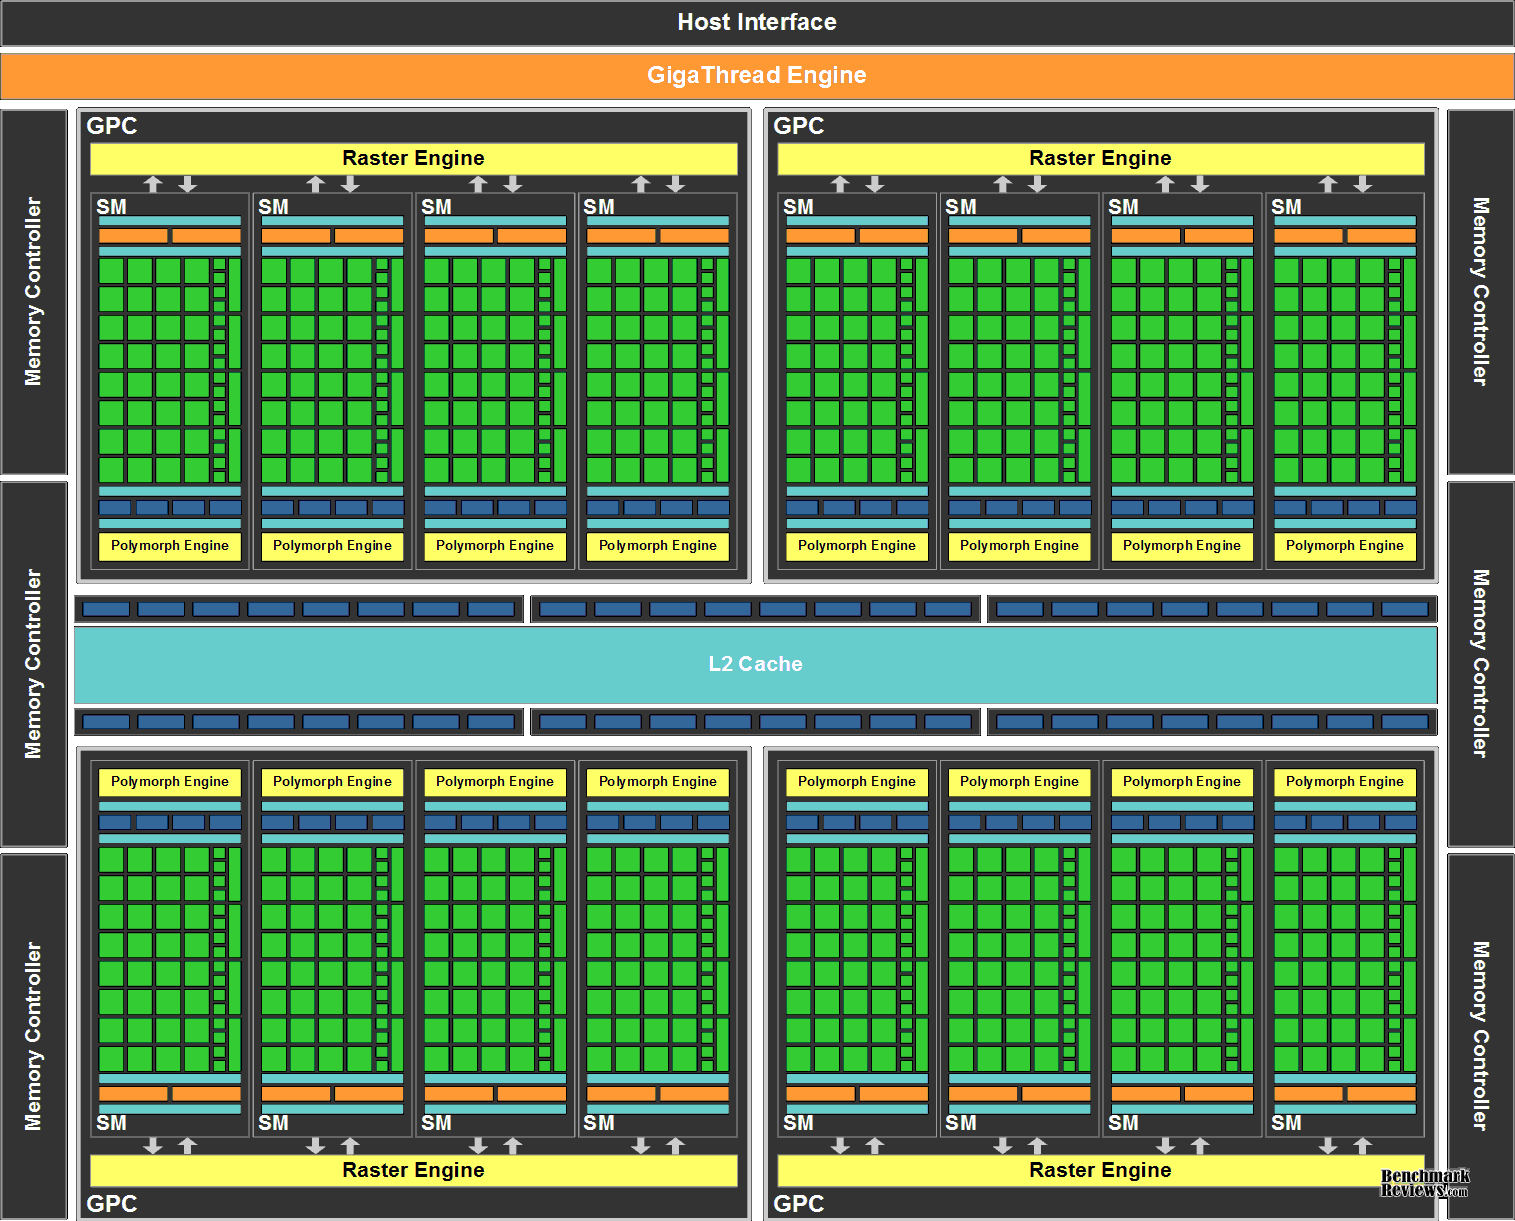
\includegraphics[width=\textwidth]{img/arq/fermi-gpu-block.pdf}
    \caption{Diagrama de bloques de GF100 Fermi. Tomado de~\cite{NvidiaFermi}.}
    \label{fermi_gpu_block}
\end{figure}

Por como funciona un pipeline gr\'afico cl\'asico, los SM se agrupan de a cuatro en GPCs (\textit{Graphics Processing Cluster}) y no interact\'ua con el modelo de c\'omputo
de CUDA.
Un esquema de esta divisi\'on global de los SM y c\'omo se comunican puede verse en la figura~\ref{fermi_gpu_block}.

%Por motivos de como funciona un pipeline gr\'afico, los SM se agrupan de 4, en un GPC (\textit{Graphics
%Processing Cluster}). Cada GPC se encarga de ejecutar los distintos pasos del pipeline gr\'afico,
%cargando a los SM con las tareas que tienen que realizar para rasterizar (es decir, convertir los
%gr\'aficos vectorialmente definidos en gr\'aficos renderizados). En aplicaciones de CUDA, estos pasos
%no importan, puesto que se trata cada SM independientemente por software.

Todos los accesos a memoria global (la memoria por fuera del procesador) se realizan a trav\'es de la cache L1 de cada SM y a trav\'es de la L2 del todo el procesador.
Esta L2 consiste de seis bancos compartidos de $128$ KB.
Estas caches se comunican de manera directa tanto con la DRAM propia de la placa como con el bus PCI Express por el cual pueden comunicarse dos placas entre s\'i, sin pasar por CPU, y son \textit{write-through}, es decir cada escritura se hace tanto en la DRAM como en la memoria cache.

%En la arquitectura Fermi, no se pueden ejecutar simult\'aneamente instrucciones de precisi\'on doble y simple y, como las de precisi\'on doble requieren ambos pipelines, suelen disminuir considerablemente el aprovechamiento de los cores.
%En la arquitectura Kepler, al usar cuatro unidades de despacho de warp, se puede elegir una mejor combinaci\'on para poder ejecutar simult\'aneamente instrucciones que no requieran usar los mismos recursos del pipeline~\cite{NvidiaKepler}.

Como estos procesadores implementan el est\'andar IEEE754-2008, cuentan con operaciones de precisi\'on simple y doble acorde al
mismo, por lo cual los c\'alculos intermedios en operaciones como FMA (\textit{Fused Multiply-Add}), que toma tres operandos y devuelve el producto de dos de ellos sumado al tercero, no pierden precisi\'on por redondeo.

%El c\'odigo escrito para CUDA se puede compilar a dos targets distintos; uno es
%el codigo binario nativo de la placa target donde se va a correr y el otro es un
%codigo intermedio, llamado c\'odigo PTX, que se JIT compila por el driver CUDA
%antes de enviar a la placa, de modo que sea portable entre placas y arquitecturas
%(retrocompatibles).

%Cuando se lanza un kernel de ejecuci\'on, este c\'odigo binario se carga en la DRAM propia
%de la placa. Este codigo va a ser ejecutado por todos los bloques que se hayan definido cuando
%se lanz\'o el kernel. El ``Thread Engine'' del GPGPU se encarga de repartir los bloques a los
%SM (Streaming Multiprocessors). Cada SM luego va a ejecutar de a grupos de 32 threads, cada uno
%de ellos corriendo sobre un SP (Streaming Processor). A traves de sus 2 o 4 unidades de dispatch de warp
%(de acuerdo a la generaci\'on de los chips), el SM puede dinamicamente cambiar el warp que se esta ejecutando en sus SP,
%escondiendo la latencia de los stalls de pipelines forzosos para la ejecucion de instrucciones de multiples clocks.
%Estos threads a su vez obtienen sus registros de un register file com\'un a todos los SP. Un scoreboard
%es mantenido por cada dispatcher de warps para poder determinar que threads estan listos para correr. En Kepler
%este scoreboard es simplificado ya que las latencias de las operaciones matem\'aticas es conocido, por
%lo cual se puede reemplazar por contadores m\'as sencillos. ~\cite{NvidiaKepler}
%Como el c\'odigo se ejecuta de manera sincr\'onica entre todos los threads del warp, las instrucciones
%condicionales proveen un problema para esta arquitectura. Como las distintas ramas del condicional
%son instrucciones excluyentes, no las deben ejecutar todos los threads simultaneamentes. El procesador
%deshabilitaba los cores que manejaban los threads de las ramas que no se ejecutaban del
%condicional~\cite{NvidiaTesla}. Para disminuir la cantidad de instrucciones de condicionales
%que se ejecutan, e cuenta con ~\cite{NvidiaFermi} predicaci\'on en todas las instrucciones de la ISA.


\section{Organizaci\'on de la memoria}

%La arquitectura CUDA esta enfocada a procesamiento de grandes cantidades de datos
%de puntos flotante. El procesador GPGPU cuenta con cientos de ALU sincronizadas
%por bloques, permitiendo un paralelismo adaptativo a distintos problemas.
%
%El procesamiento GPGPU es similar al procesamiento vectorial
%realizado por las supercomputadoras Cray y IBM que surgio en los 1960's, pero
%en vez de usar VLIW para procesamiento masivo, CUDA usa multiples hilos de ejecuci\'on
%que trabajan simultaneamente sobre los datos.
%El procesamiento consiste en un funcionamiento hibrido entre compilador y procesador. Se determina
%un conjunto de elementos a procesar y se elije de manera explicita una manera de particionar el
%problema a la hora de ser enviado para procesado a la placa.
%
%Para realizar el computo, esta arquitectura cuenta a su vez con multiples clases de memorias
%que se adaptan de maneras diferentes a los distintos procesos. Estas incluyen:

La memoria de la GPU es uno de los puntos cruciales de esta arquitectura, un esquema gr\'afico puede observarse en la figura~\ref{fig:cuda-memories}.
Esta se subdivide entre memorias on-chip y memorias on-board, de acuerdo a su ubicaci\'on y latencia de acceso, en cuatro categor\'ias distintas:

\begin{itemize}
  \item Registros
  \item Memoria local
  \item Memoria compartida
  \item Memoria global
\end{itemize}

Cada \thread{} de ejecuci\'on cuenta con una cantidad limitada de registros de punto flotante de $32$ bits con latencia de un par de ciclos de clock.
A su vez, existe una cantidad finita de registros totales que cuenta un SM (oscila entre $16535$ y $65535$ registros).
Por su baja latencia son la clase principal de almacenamiento temporal.

La memoria local es una memoria propia de cada \thread{}, y se encuentra almacenada dentro de la memoria global.
Esta memoria es definida autom\'aticamente por el compilador y sirve como \'area de almacenamiento cuando se acaban los registros: los valores anteriores se escriben a esta memoria, dejando los registros libres para nuevos valores en c\'alculos, y cuando se terminan estos c\'alculos se carga los valores originales nuevamente.
Cuenta con las mismas desventajas que la memoria global, incluyendo su tiempo de acceso.

La memoria compartida, o \textit{shared}, es una memoria que es visible para todos los \threads{} dentro de un mismo SM.
Cada \thread{} puede escribir en cualquier parte de la memoria compartida dentro de su bloque y puede ser le\'ido por cualquier otro \thread{} de este.
Es una memoria muy r\'apida, on-chip, y que tarda aproximadamente $40$ ciclos de acceso~\cite{Demystifying}.
Esta memoria es compartida con la cache L1, la cual tiene capacidad de entre $16$ KB y $64$ KB configurable por software.
Esta memoria se encuentra dividida en $32$ bancos de $2$ KB de tama\~no, permitiendo que cada uno de los $32$ \threads{} acceda independientemente a un float.
Si hubiera conflicto, los accesos a ese banco se serializar\'ian, aumentando la latencia de la llamada~\cite{farberCuda}.

La memoria global es la memoria principal fuera del chip de la GPU.
Esta es de gran tama\~no (de entre $1$ GB y $12$ GB) y es compartida por todos los SM de la GPU y los CPU que integran el sistema.
Es decir, tanto los GPU como los CPU pueden invocar las funciones de CUDA para transferir datos entre la memoria de la placa y la memoria RAM de \textit{host}.
La latencia de acceso a la memoria global es de cientos de ciclos~\cite{Demystifying}, sumamente lenta en comparaci\'on con el procesador.
La memoria global tambi\'en puede ser mapeada, o \textit{pinneada}, para que exista una copia de esa reserva tanto en la memoria en la placa como en la memoria principal del procesador. El driver de CUDA va a mantener la consistencia entre ambas de manera as\'incrona, evitando la necesidad de hacer copias de memoria expl\'icitas.
No es ilimitada la cantidad de memoria mapeada posible, por lo que es importante saber elegir qu\'e elementos se van a almacenar de esta manera.

\begin{figure}[htb]
    \centering
    \includegraphics[width=250px]{img/arq/cuda-memories_ES.pdf}
    \caption{Esquema de la jerarqu\'ia de memorias en GPU, detallando de las disponibles en cada SM, la memoria compartida (SMEN), la L2 global, la
    memoria de la placa (global) y la mapeada entre el \textit{host} y la placa de video. Tomado de~\cite{farberCuda}.}
    \label{fig:cuda-memories}
\end{figure}

Adicionalmente, la GPU cuenta con m\'ultiples niveles de memorias cache para poder aminorar el hecho de que el principal cuello de botella del c\'omputo es la latencia en los accesos a memoria global.
Estas se dividen en cuatro:

\begin{itemize}
  \item Cache L1
  \item Cache L2
  \item Cache constante
  \item Cache de textura
\end{itemize}

La cache L1 es dedicada por SM.
Esta cache fue introducida en Fermi y su dise\~no hace que tambi\'en est\'a dedicada a la memoria compartida, por lo que es posible en tiempo de ejecuci\'on darle directivas a la GPU que asigne m\'as memoria cache o m\'as memoria compartida, permitiendo a los bloques tener mayores espacios de memorias compartidas o mayores \textit{hit rates} de caches.

La cache L2 es com\'un a todos los SM de la GPU, donde, a partir de Fermi en \nvidia{}, todos los accesos de lectura y escritura a memoria global y textura pasan a trav\'es de esta~\cite{NvidiaFermi}.

La cache constante es una cache sobre la memoria global dedicada solamente a lecturas de memoria.
Esta es muy reducida (solo cuenta con $64$ KB) y est\'a optimizada para muchos accesos a la misma direcci\'on.
Cuando un \thread{} lee esta memoria, se retransmite a los dem\'as \threads{} del warp que est\'en leyendo esa misma direcci\'on, reduciendo el ancho de banda necesario.
Si, en cambio, los \threads{} leen distintas direcciones, los accesos se serializan.
Cuando hay un \emph{miss} de esta memoria, la lectura tiene el costo de una lectura de memoria global.

La cache de textura es una cache sobre la memoria global que presenta no solo localidad espacial, como la mayor\'ia de las caches de procesadores normales (es decir, la cache contiene una porci\'on consecutiva de la memoria principal), sino que se le puede agregar el concepto de dimensiones, para poder modelar datos en m\'as de una dimensi\'on.
Esto se adapta de muy bien a los problemas de gr\'aficos en 2D y 3D, y es una herramienta clave a la hora de minimizar los accesos a matrices no solo por filas sino por columnas.
Esta cache se debe definir en momento de compilaci\'on en el c\'odigo, ya que tiene l\'imites espaciales (necesarios para poder definir \'areas de memoria sobre la cual operar) y a su vez se debe acceder a los datos subyacentes a trav\'es de funciones espec\'ificas.
Una caracter\'istica adicional de esta cache es que como necesita resolver estos accesos no convencionales a la memoria, cuenta con una unidad propia de resoluci\'on de direcciones. Esta unidad tiene limitantes en cuanto a sus posibilidades, ya que no posee un ancho de banda suficiente como para resolver todos los accesos a memoria globales que podr\'ian surgir, por lo cual su uso debe ser criterioso.


\section{Esquema de paralelismo}

Al ser una arquitectura masivamente paralela desde su concepci\'on, CUDA presenta varios niveles de paralelismo, para agrupar l\'ogicamente el c\'omputo y poder dividir f\'isicamente su distribuci\'on.
Los principales son:
\begin{itemize}
  \item Bloques de \threads{}
  \item Grilla de bloques
  \item Streams
  \item M\'ultiples placas
\end{itemize}

El paralelismo a nivel de bloque instancia una cantidad de \threads{}, subdivididos l\'ogicamente en 1D, 2D o 3D.
Los \threads{} internamente se agrupan de a $32$, es decir, un \textit{warp}.
Cada uno de estos \threads{} va a contar con una manera de identificarlos un\'ivocamente: un \texttt{blockId} y, dentro de cada bloque, su propio \texttt{threadId}.
Adem\'as, van a correr simult\'aneamente en el mismo SM y van a ser puestos y sacados de ejecuci\'on de a un warp din\'amicamente por el \textit{scheduler} de hardware que cuenta cada SM.
Para compartir informaci\'on entre ellos, se puede utilizar la memoria compartida o las instrucciones de comunicaci\'on de \threads{} intrawarp (solo disponibles a partir de Kepler~\cite{NvidiaKepler}).

El paralelismo a nivel de grilla determina una matriz de bloques de ejecuci\'on que particiona el dominio del problema.
El \emph{GigaThread Scheduler} va a ejecutar cada bloque en un SM hasta el final de la ejecuci\'on de todos los \threads{} de este.
Los bloques no comparten informaci\'on entre s\'i. Por esto, no pueden ser sincronizados mediante memoria global ya que no se asegura el orden en el que ser\'an puestos a correr, y un bloque mantiene su SM ocupado hasta que termine de ejecutar, bloqueando a los dem\'as (es decir, no hay \textit{preemption} en los SM).

El paralelismo de stream es una herramienta empleada para hacer trabajos concurrentes usando una sola placa.
Esta t\'ecnica permite que m\'ultiples kernels (unidades de c\'odigo en CUDA) o copias de memoria independientes est\'en encolados, para que el driver pueda ejecutarlas simult\'aneamente si se est\'an subutilizando los recursos, de forma de minimizar tiempo ocioso del dispositivo.
Los streams permiten kernels concurrentes pero cuentan con importantes restricciones que generan sincronizaci\'on impl\'icita, lo cual hay que tener presente si se desea mantener el trabajo de forma paralela.

El paralelismo a nivel de placa consiste en poder distribuir la carga del problema entre distintas GPUs dispuestas en un mismo sistema compartiendo una memoria RAM com\'un como si fuera un software multithreaded tradicional.
CUDA no cuenta con un modelo impl\'icito de paralelismo entre distintas placas, pero es posible hacerlo manualmente eligiendo de manera expl\'icita qu\'e dispositivo usar.
Las placas se pueden comunicar as\'incronamente entre s\'i, tanto accediendo a las memorias globales de cada una como ejecutando c\'odigo remotamente.
En las versiones modernas del driver de CUDA, tambi\'en pueden comunicarse directamente las placas entre s\'i a trav\'es de la red, permitiendo escalar multinodo f\'acilmente en un cluster de c\'omputo~\cite{farberCuda}.

\section{Diferencias entre Tesla, Fermi, Kepler}

Hasta ahora se describi\'o la arquitectura vista desde el punto de vista Fermi, que es la segunda arquitectura GPGPU dise\~nada por \nvidia{}.
Fermi es la evoluci\'on de Tesla, construida para desacoplar a\'un m\'as los conceptos de procesamiento gr\'afico de modo de lograr un procesador m\'as escalable y de prop\'osito general.
La arquitectura sucesora a Fermi es Kepler, presentada en el 2012, con las metas de disminuir el consumo y aumentar la potencia de c\'alculo~\cite{NvidiaKepler}.

\begin{table}[h]
  \begin{tabular}{@{}llll@{}}
  \toprule
  Caracter\'isticas        & Tesla (GT200)   & Fermi (GF100)   & Kepler (GK110)   \\ \midrule
  A\~no introducci\'on     & 2006            & 2010            & 2012             \\
  Transistores             & 1400 millones   & 3000 millones   & 3500 millones    \\
  Tecnolog\'ia fabricaci\'on & 65 nm           & 40 nm           & 28 nm            \\
  SMs                      & 30              & 16              & 15               \\
  SP / SM                  & 8               & 32              & 192              \\
  Cach\'e L1               & -               & 16 - 48 KB       & 16 - 32 - 48 KB   \\
  Cach\'e L2               & -               & 768 KB           & 1536 KB           \\
  Memoria Shared/SM      & 16 KB            & 16 - 48 KB       & 16 - 32 - 48 KB   \\
  Registros/Thread         & 63              & 63              & 255              \\
  Pico Precisi\'on Simple    & 240 MAD / clock & 512 FMA / clock & 2880 FMA / clock \\
  Pico GFLOPS Simple       & 933             & 1345            & 3977             \\
  GFLOPS/Watt              & $3.95$            & $5.38$            & $15.9$             \\ \bottomrule
  \end{tabular}
\caption{Tabla comparativa de las caracter\'isticas m\'as prominentes de las tres arquitecturas de CUDA.}
\label{tab:CudaGenerations}
\end{table}

En la tabla \ref{tab:CudaGenerations} se ve una comparaci\'on de las recursos que est\'an m\'as directamente relacionados a la \performance{} de un dispositivo GPU.
Se puede apreciar el crecimiento notable del poder de c\'omputo debido a las tecnolog\'ias de fabricaci\'on, que permitieron aumentar la cantidad de transistores por unidad de superficie.
Tambi\'en se puede comprobar que, a diferencia de los CPU, las arquitecturas GPGPU decidieron utilizar esos nuevos transistores disponibles para m\'as n\'ucleos de procesamiento, en vez
de dedicarlas a aumentar las memorias cache, que crecieron m\'inimamente (comparando contra las caches de CPU).

Una de las diferencias m\'as notorias entre Tesla y Fermi es la presencia de FMA contra el MAD (\textit{Multiply - Add}).
El MAD realiza la multiplicaci\'on y la acumulaci\'on en dos pasos, pero m\'as r\'apidos que hacerlos independientemente por tener hardware dedicado.
Debido a que debe redondear entre los pasos, pierde precisi\'on y no respeta completamente el est\'andar IEEE754-2008.
El FMA, en cambio, lo hace en una sola operaci\'on, y sin redondeos intermedios.

La m\'etrica usada por \nvidia{} para publicitar la \performance{} de estos dispositivos y poder compararlos entre s\'i, y contra CPU, son los GFLOPS.
Esta unidad mide cuantas operaciones de punto flotante de precisi\'on simple se pueden realizar por segundo.
Los GFLOPs son utilizados tambi\'en por los clusters en el ranking TOP500, donde se ordenan de acuerdo a la \performance{} medida usando un software estandarizado, \texttt{LINPACK}.
No solo es notable como se cuadruplic\'o la \performance{} (te\'orica) en solamente seis a\~nos, sino que a\'un m\'as importante es como mejor\'o la \performance{} por Watt.
Esto tambi\'en se ve en que Kepler tiene menos SM que Fermi o Tesla, pero son mucho m\'as poderosos y eficientes.
La tecnolog\'ia de fabricaci\'on ha ayudado a la disminuci\'on del consumo, un problema que acechaba a los dise\~nos Fermi, ya que sus consumos superiores a 200W por dispositivo los hac\'ian muy dif\'iciles de refrigerar incluso en clusters de HPC.
Se puede apreciar entonces la estrategia de mercado de \nvidia{} de introducirse en las supercomputadoras de todo el mundo, donde el consumo y la refrigeraci\'on son factores limitantes (mucho m\'as a\'un que, por ejemplo, en computadoras de escritorio)~\cite{HennessyPatterson}.

\section{CUDA, Herramientas de desarrollo, profiling, exploraci\'on}

Para soportar una arquitectura masivamente paralela, se debe usar una ISA (\textit{Instruction Set Architecture}) dise\~nada especialmente para el problema.
En el caso de CUDA, esta ISA se denominada PTX y debe poder soportar conceptos fundamentales del c\'omputo GPGPU: grandes cantidades de registros, operaciones en punto flotante de precisi\'on simple y doble, y FMA~(fused multiply-add).
Adem\'as, el c\'odigo compilado para GPU debe ser agn\'ostico al dispositivo que lo va a correr, por lo cual la paralelizaci\'on no debe estar demasiado atada a este, sino que el dispatching lo debe poder determinar el driver de la placa en tiempo de ejecuci\'on.
Un \'ultimo requerimiento clave de esta ISA es que debe soportar hacer ajustes manuales, para poder construir partes claves de ciertas bibliotecas frecuentemente usadas (como las
rutinas de BLAS de \'algebra lineal)~\cite{NvidiaFermi}.

El lenguaje CUDA es una extensi\'on de C++, con ciertas caracter\'isticas agregadas para poder expresar la subdivisi\'on de las rutinas en \threads{} y bloques, junto con mecanismos para especificar qu\'e variables y funciones van a ejecutarse en la GPU y en el CPU.
Una caracter\'istica de CUDA es que todas las llamadas a los kernels de ejecuci\'on son asincr\'onicas, por lo que es relativamente sencillo solapar c\'odigo en GPU y CPU.
A su vez se cuenta con m\'ultiples funciones opcionales, con distinta granularidad, que permiten esperar a que todas las llamadas as\'incronas a GPU finalicen, agregando determinismo
en forma de barreras de sincronizaci\'on al lenguaje.

El c\'odigo CUDA compila usando \texttt{nvcc}, una variante del \texttt{GNU gcc} que se encarga de generar el c\'odigo PTX para las funciones que se van a ejecutar en las GPU.
Este c\'odigo objeto despu\'es se adosa normalmente con el resto del c\'odigo que corre en CPU y se genera un binario ejecutable.

\nvidia{}, adem\'as, provee herramientas de profiling para explorar c\'omo se est\'an utilizando los recursos durante la ejecuci\'on.
\'Estas son esenciales para optimizar, puesto que los limitantes de GPU son sumamente distintos a los de CPU, presentando dificultades conceptuales incluso para programadores experimentados.
Las herramientas de profiling no solo muestran \emph{runtime}, sino que sirven para ver d\'onde hay accesos a memoria excesivos, puntos de sincronizaci\'on costosos, limitantes en los registros y c\'omo se superponen las llamadas asincr\'onicas.

El uso de todas estas herramientas fue vital en este trabajo para poder entender c\'omo funciona la arquitectura en detalle, c\'omo medir \performance{} y utilizaci\'on, y c\'omo los cambios realizados impactaron en las distintas generaciones de dispositivos.

\section{Requerimientos de un problema para GPGPU}

Dada la organizaci\'on de un procesador GPU, un problema debe exhibir al menos las siguientes caracter\'isticas para que tenga potencialidad para poder aprovechar las caracter\'isticas y recursos disponibles en esta arquitectura:

\begin{enumerate}
  \item \label{req:paralelo} El problema debe tener una gran parte paralelizable.
  \item \label{req:float} El problema debe consistir, mayormente, de operaciones num\'ericas.
  \item \label{req:matrix} El problema debe poder ser modelado, en su mayor parte, utilizando arreglos o matrices.
  \item \label{req:transf} El tiempo de c\'omputo debe ser muy superior al tiempo de transferencia de datos.
\end{enumerate}

El \'item \ref{req:paralelo} se refiere a que debe existir alguna forma de partir el problema en subproblemas que puedan realizarse simult\'aneamente, sin que haya dependencias de
resultados entre s\'i.
Si el problema requiere partes seriales, lo ideal es que se las pueda dividir en partes independientes que sean etapas de una cadena de procesos, donde cada una de \'estas exhiban caracter\'isticas fuertemente paralelas.
Como las arquitecturas masivamente paralelas tienen como desventaja una menor eficiencia por n\'ucleo, si el problema no se puede dividir para maximizar la ocupaci\'on de todos los procesadores disponibles, va a resultar muy dif\'icil superar en eficiencia a los procesadores seriales.

El ítem~\ref{req:float} habla acerca de que el m\'etodo de resoluci\'on de los problemas debe provenir de una aplicaci\'on num\'erica o de gran carga aritm\'etica.
El set de instrucciones de las arquitecturas GPGPU est\'an fuertemente influenciados por las aplicaciones 3D que las impulsaron en un principio.
\'Estas consisten mayormente de transformaciones de \'algebra lineal para modelar iluminaci\'on, hacer renders o mover puntos de vistas.
Todos estos problemas son inherentemente de punto flotante, por lo cual el set de instrucciones, las ALUs internas y los registros est\'an optimizados para este caso de uso.

El ítem \ref{req:matrix} menciona que los problemas que mejor se pueden tratar en esta arquitectura se pueden representar como operaciones entre arreglos o matrices de dos, tres o cuatro dimensiones.
Las estructuras de datos no secuenciales en memoria incurren en m\'ultiples accesos a memoria para recorrerlas y, en las arquitecturas GPGPU, generan un gran cuello de botella.
Adem\'as, suelen ser dif\'iciles de paralelizar en m\'ultiples subproblemas.
Tener como par\'ametros de entrada matrices o arreglos que se puedan partir f\'acilmente producen en overheads m\'inimos de c\'omputo y permiten aprovechar mejor las memorias caches y las herramientas de prefetching que brinda el hardware.

El \'item \ref{req:transf} ataca uno de los puntos cr\'iticos de esta arquitectura.
Para poder operar con datos, se requiere que est\'en en la memoria de la placa, no en la memoria de prop\'osito general de la computadora.
Se debe, entonces, hacer copias expl\'icitas entre las dos memorias, ya que ambas tienen espacios de direcciones independientes.
Esta copia se realiza a trav\'es de buses que, a pesar de tener un gran \emph{throughput}, tambi\'en tienen una gran latencia (del orden de milisegundos).
Por lo tanto, para minimizar el tiempo de ejecuci\'on de un programa usando GPGPUs, se debe considerar tambi\'en el tiempo de transferencia de datos a la hora de determinar si el beneficio de computar en menor tiempo lo justifica.
Las nuevas versiones de CUDA buscan brindar nuevas herramientas para simplificar este requerimiento, proveyendo espacio de direccionamiento \'unico y memoria unificada~\cite{farberCuda}, pero siguen siendo copias de memoria a trav\'es de los buses (aunque asincr\'onicas).

Estas caracter\'isticas limitan enormemente la clase de problemas que una GPGPU puede afrontar, y suelen ser una buena heur\'istica para determinar de antemano si vale la pena
invertir el tiempo necesario para la implementaci\'on y ajuste fino.

\section{Diferencia entre CPU y GPU - Procesadores especulativos}

Hasta ahora, solo se consideraron a los GPUs de forma aislada, observando las prestaciones del hardware y una aproximaci\'on a la manera en que se escriben los programas para esta arquitectura.
La esencia de GPGPU se puede apreciar mejor compar\'andola contra los motivos de la evoluci\'on de CPU, y los problemas que se fueron enfrentando los dise\~nos siguiendo la historia de los componentes que fueron apareciendo en estos.
% Esto se mostr\'o en la tabla \ref{tbl:historia-cpu} (p\'agina~\pageref{tbl:historia-cpu}), que detalla algunos de los eventos m\'as importantes que aceleraron
% la \performance{} de los CPU.

Lo clave es observar el siguiente patr\'on: \emph{``no desechar algo que pudi\'eramos necesitar pronto''}, \emph{``intentar predecir el futuro de los condicionales''}, \emph{``intentar correr m\'ultiples instrucciones a la vez porque puede llegar a bloquear en alguna de ellas''}.

Todos estos problemas han convertido al CPU en un dispositivo que gira alrededor de la especulaci\'on, de los valores futuros que pueden tener las ejecuciones, del probable reutilizaci\'on de datos.
En un CPU moderno (por ej. Intel Xeon E7-8800~\cite{XeonE78800Spec}) las unidades que verdaderamente realizan las operaciones l\'ogico-aritm\'eticas (las ALU) son muy pocas en comparaci\'on con la cantidad utilizadas para las operaciones de soporte.

En contraste, los dispositivos GPU son verdaderos procesadores de c\'omputo masivo.
Est\'an dise\~nadas para resolver constantemente operaciones muy bien definidas (instrucciones de punto flotante en su mayor\'ia).
Comparativamente con un CPU, las ALU de las GPU son bastante pobres y lentas.
No funcionan a las mismas velocidades de clock (rara vez superan $1.1$ GHz) y sus SP deben estar sincronizados entre s\'i.
Pero la gran ventaja esta en la cantidad.

Un CPU cuenta con pocas ALU por core, dependiendo de la cantidad de cores y del tama\~no de sus operaciones SIMD (alrededor de $16$ cores por \emph{die} de x86 es el tope de l\'inea ofrecido actualmente, procesando de a $32$ bytes simult\'aneamente).
Un GPU cuenta con miles de ALUs en total (m\'as de $2500$ CUDA cores en una Tesla K20~\cite{NvidiaKeplerDatasheet}).
El dise\~no de esta arquitectura concibe la escalabilidad cuantitativa de las unidades de c\'omputo como la caracter\'istica esencial a tener, tanto por su \'enfasis fundamental, las aplicaciones gr\'aficas, como para su aspecto de coprocesador num\'erico de prop\'osito general.

Por contrapartida, los GPUs disponen de pocas unidades de soporte del procesamiento.
\'Estos no disponen de pipelines especulativos, el tama\~no de las caches est\'an a \'ordenes de magnitud de las de CPU, la latencia a las memorias principales de la GPU est\'an a centenas de clocks de distancia, etc.
La arquitectura supone que siempre va a tener m\'as trabajo disponible para realizar, por lo cual en vez de intentar solucionar las falencias de un grupo de \threads{}, directamente
pone al grupo en espera para m\'as adelante y contin\'ua procesando otro warp de \threads{}.
Se puede notar que durante del dise\~no de la arquitectura CUDA, buscaron resolver el problema del c\'omputo masivo pensando en hacer m\'as cuentas a la vez y recalcular datos, si fuera necesario.
Esto es una marcada diferencia con respecto a los CPU, que est\'an pensados en rehacer el menor trabajo posible e intentar mantener todos los datos que pueda en las memorias caches masivas.

Nuevamente, en este punto se puede apreciar el legado hist\'orico de los CPU.
Al tener que poder soportar cualquier aplicaci\'on, no pueden avocarse de lleno a una sola problem\'atica.
Para las arquitecturas GPGPU, el hecho de no tener que dise\~nar un procesador de prop\'osito general compatible con versiones anteriores, permiti\'o un cambio radical a la hora de concebir una arquitectura de gran throughput auxiliar al procesador, no reemplaz\'andolo sino m\'as bien adicionando poder de c\'omputo~\cite{GlaskowskyFermi}.

Las arquitecturas Tesla, Fermi y Kepler conciben el dise\~no de un procesador de alto desempe\~no.
Su meta principal es poder soportar grandes cantidades de paralelismo, mediante el uso de procesadores sim\'etricos, pero tomando la fuerte restricci\'on de \textsl{``no siempre tiene que andar bien''}.
Es decir, los dise\~nadores suponen que el c\'odigo que van a ejecutar esta bien adaptado a la arquitectura y no disponen casi de mecanismos en el procesador para dar optimizaciones post-compilaci\'on.
Relajar esta restricci\'on permite romper con el modelo de c\'omputo de CPU y definir nuevas estrategias de paralelismo, que no siempre se adaptan bien a todos los problemas, pero para el subconjunto de los desaf\'ios que se presentan en el \'area de HPC y de v\'ideo juegos han probado ser un cambio paradigm\'atico.

\section{Idoneidad para la tarea}

El método de dinámica molecular tratado en este trabajo es un problema que implica una gran cantidad de operaciones matemáticas de gran volumen de cálculos e independientes entre si.
El cálculo de fuerzas, la suma de todas las fuerzas parciales y la actualización de coordenadas son todos cálculos que se deben resolver para todas las partículas de forma individual. 
Esto implica una gran cantidad de cálculos pero además una gran cantidad de datos que deben ser actualizados en cada paso de la simulación.
En particular, la gran cantidad de accesos necesarios para actualizar constantemente los datos asociados a cada partícula constituye un cuello de botella en este tipo de aplicaciones.

Dadas las caracter\'isticas de contar con un fuerte nivel de paralelismo y de ser operaciones mayormente de punto flotante, hace ya algún tiempo 
las arquitecturas GPU se convirtieron en estándar para la aplicación de métodos de DM, tal como se vió en el capítulo 1.

% De todas formas, aún queda mucho por avanzar. 


% se determin\'o que el uso de GPGPU para este problema era promisorio, en comparaci\'on con arquitecturas de prop\'osito general con menos poder de c\'omputo. 


% 
% El problema de QM/MM enfrentado en este trabajo cuenta con m\'ultiples operaciones matem\'aticas de gran volumen de c\'alculos.
% En particular, las operaciones matriciales constituyen los principales cuellos de botella en esta aplicaci\'on.
% Estas operaciones se realizan para varios grupos dentro de una grilla de integraci\'on (ecuaci\'on~\ref{eq:xc}), los cuales se pueden realizar de manera independiente (y por lo tanto en paralelo).
% 
% Para obtener los valores num\'ericos de densidad buscados en los puntos, se deben obtener las derivadas primeras y segundas, lo cual implica hacer m\'ultiples operaciones de multiplicaci\'on matricial.
% Este tipo de problemas est\'a estudiado fuertemente en la literatura debido a la multiplicidad de aplicaciones de diferentes campos que requieren de operaciones de \'algebra lineal.
% 
% En nuestro caso, para un sistema se requieren miles de estas multiplicaciones entre matrices, algunas con matrices de m\'as de $500^2$ elementos.
% Como LIO es un proyecto de resoluci\'on num\'erica de QM/MM, los problemas enfrentados son casi, en su totalidad, operaciones de punto flotante.
% Luego, dadas las caracter\'isticas de contar con un fuerte nivel de paralelismo en los cuellos de botella y de ser operaciones mayormente de punto flotante, 
% se determin\'o que el uso de GPGPU para este problema era promisorio, en comparaci\'on con arquitecturas de prop\'osito general con menos poder de c\'omputo. 
% La exploraci\'on original de esta arquitectura trajo buenos resultados, por lo que se prosigui\'o su an\'alisis como un camino prometedor~\cite{TesisNitsche}.

% \chapter{La arquitectura GPU}

\section{Introducci\'on}

Este trabajo se centra en la arquitectura GPU desarrollada por \nvidia{}, conocida como CUDA por las siglas en ingles de \textit{Compute Unified Device Architecture}.
CUDA surge naturalmente de la aplicaci\'on del hardware desarrollado para problemas gr\'aficos, pero aplicados al c\'omputo cient\'ifico.

Las placas de v\'ideo aparecen en 1978 con la introducci\'on de Intel del chip \texttt{iSBX 275}.
En 1985, la Commodore Amiga inclu\'ia un coprocesador gr\'afico que pod\'ia ejecutar instrucciones independientemente del CPU, un paso importante en la separaci\'on y especializaci\'on de las tareas.
En la d\'ecada del 90, m\'ultiples avances surgieron en la aceleraci\'on 2D para dibujar las interfaces gr\'aficas de los sistemas operativos y, para mediados de la d\'ecada, muchos fabricantes estaban incursionando en las aceleradoras 3D como agregados a las placas gr\'aficas tradicionales 2D.
A principios de la d\'ecada del 2000, se agregaron los \textit{shaders} a las placas, peque\~nos programas independientes que corr\'ian nativo en el GPU, y se pod\'ian encadenar entre s\'i, uno por pixel en la pantalla~\cite{Mark2003}.
Este paralelismo es el desarrollo fundamental que llev\'o a las GPU a poder procesar operaciones gr\'aficas \'ordenes de magnitud m\'as r\'apido que el CPU.

En el 2006, \nvidia{} introduce la arquitectura G80, que es el primer GPU que deja de resolver \'unicamente problemas de gr\'aficos para pasar a un motor gen\'erico donde cuenta con un set de instrucciones consistente para todos los tipos de operaciones que realiza (geometr\'ia, vertex y pixel shaders)~\cite{cudaHandbook}.
Como subproducto de esto, la GPU pasa a tener procesadores sim\'etricos m\'as sencillos y f\'aciles de construir.
Esta arquitectura es la que se ha mantenido y mejorado en el tiempo, permitiendo a las GPU escalar masivamente en procesadores simples, de baja frecuencia de reloj y con una disipaci\'on t\'ermica manejable.

Los puntos fuertes de las GPU modernas consisten en poder atacar los problemas de paralelismo de manera pseudo-expl\'icita, y con esto poder escalar ``f\'acilmente'' si solamente se corre en una placa con m\'as procesadores~\cite{cudaProgrammingGuide}.

T\'ecnicamente, esta arquitectura cuenta con entre cientos y miles de procesadores especializados en c\'alculo de punto flotante, procesando cada uno un \textit{thread} distinto pero
trabajando de manera sincr\'onica agrupados en bloques.
Cada procesador, a su vez, cuenta con entre $63$ a $255$ registros~\cite{NvidiaFermi,NvidiaKepler}.
Las GPU cuentas con m\'ultiples niveles de cache y memorias especializadas (subproducto de su dise\~no fundamental para gr\'aficos).
Estos no poseen instrucciones SIMD, ya que su dise\~no primario esta basado en cambio, en SIMT (\textit{Single Instruction Multiple Thread}), las cuales se ejecutan en los bloques sincr\'onicos de procesadores.
De este modo, las placas modernas como la \nvidia{} Tesla K40 alcanzan poder de c\'omputo de $4.3$ TFLOPs (4300 mil millones de operaciones de punto flotante por segundo) en c\'alculos de precisi\'on simple, $1.7$ TFLOPs en precisi\'on doble y $288$ GB/seg de transferencia de memoria, usando $2880$ CUDA Cores~\cite{NvidiaKeplerDatasheet}.
Para poner en escala la concentraci\'on de poder de c\'alculo: una computadora usando solo dos de estas placas posee una capacidad
de c\'omputo comparable a la supercomputadora m\'as potente del mundo en Noviembre 2001~\cite{Top500November2001}.
Una comparativa del poder de c\'omputo te\'orico entre GPUs y CPUs puede ver en la figura~\ref{fig:cuda-gflops}.

\begin{figure}[htbp]
    \centering
    \includegraphics[width=\plotwidthsmaller]{img/arq/cuda-gflops_ES.pdf}
    \caption{Picos te\'oricos de \performance{} en GFLOPS/s. Tomado de~\cite{cudaProgrammingGuide}.}
    \label{fig:cuda-gflops}
\end{figure}

Para poder explotar la arquitectura CUDA, los programas deben ser dise\~nados de manera de que el problema se pueda particionar usando el modelo de grilla de bloques de \threads{}.
Para este prop\'osito es que \nvidia{} desarroll\'o el lenguaje CUDA.

Hoy en d\'ia, poder aprovechar la potencialidad de las GPU requiere una reescritura completa de los c\'odigos ya existentes desarrollados para CPU y un cambio de paradigma importante, al dejar de tener vectorizaci\'on, paralelizaci\'on autom\'atica y otras t\'ecnicas tradicionales de optimizaci\'on en CPU.
Sin embargo, este trabajo ha rendido sus frutos en muchos casos: en los \'ultimos seis a\~nos, la literatura de HPC con aplicaciones en GPU ha explotado con desarrollos nuevos basados en la aceleraci\'on de algoritmos num\'ericos (su principal uso). Por este motivo, este trabajo no ahondar\'a
en las particularidades del lenguaje CUDA y su modelo de paralelismo, m\'as all\'a de lo estrictamente necesario para analizar \performance{}. Para m\'as informaci\'on se puede consultar la bibliografia~\cite{cudaHandbook,farberCuda,CudaOverview}.

Adem\'as, no todas las aplicaciones deben reescribirse de manera completa.
Con la introducci\'on de las bibliotecas \texttt{CuBLAS} y \texttt{CuFFT}, se ha buscado reemplazar con m\'inimos cambios las hist\'oricas bibliotecas \texttt{BLAS} y \texttt{FFTw}, piedras fundamentales del c\'omputo HPC~\cite{cublas,cufft}.

Nuevas soluciones para la portabilidad se siguen desarrollando: las bibliotecas como \texttt{Thrust}~\cite{thrust}, \texttt{OpenMP} 4.0~\cite{OpenMPSpec} y \texttt{OpenACC} 2.0~\cite{OpenACCSpec} son herramientas que buscan generar c\'odigo que puedan utilizar eficientemente el acelerador de c\'omputo que se haya disponible.
Estas herramientas permiten definir las operaciones de manera gen\'erica y dejan el trabajo pesado al compilador para que subdivida el problema de manera que el acelerador (CPU, GPU, MIC) necesite.
Obviamente, los ajustes finos siempre quedan pendiente para el programador especializado, pero estas herramientas representan un avance fundamental al uso masivo de t\'ecnicas de paralelizaci\'on autom\'aticas, necesarias hoy d\'ia y potencialmente imprescindibles en el futuro.

\section{Organizaci\'on de procesadores}

Los procesadores GPGPU dise\~nados por \nvidia{} han sido reorganizados a lo largo de su existencia m\'ultiples veces pero conservan algunas l\'ineas de dise\~no a trav\'es de su evoluci\'on.
A continuaci\'on se describe la organizaci\'on definida en la arquitectura \texttt{Fermi} y luego analizaremos las diferencias con \texttt{Kepler}.

Las arquitecturas de las GPUs se centran en el uso de una cantidad escalable de procesadores \textit{multithreaded} denominados \textit{Streaming Multiprocessors}~(SMs).
Un multiprocesador esta dise\~nado para ejecutar cientos de threads concurrentemente, usando sus unidades aritm\'eticas llamadas \textit{Streaming Processors}~(SPs).
Las instrucciones se encadenan para aprovechar el paralelismo a nivel instrucci\'on dentro de un mismo flujo de ejecuci\'on, y funcionando en conjunto con el paralelismo
a nivel de \thread{}, usado de manera extensa a trav\'es del hardware.
Todas las instrucciones son ejecutadas en orden y no hay predicci\'on de saltos ni ejecuci\'on especulativa, todo se ejecuta solamente cuando se lo necesita~\cite{CudaOverview}.

\begin{figure}[htb]
    \centering
    \includegraphics[width=0.5\textwidth]{img/arq/fermi-sm.pdf}
    \caption{Diagrama de bloques del SM de GF100 Fermi. Basado en~\cite{NvidiaFermi}.}
    \label{fermi_sm}
\end{figure}

Los SMs (figura~\ref{fermi_sm}) son unidades completas de ejecuci\'on.
Cada uno de ellos tiene $32$ SPs interconectados entre s\'i que operan sobre un \emph{register file} de $64$ KB com\'un a todos.
Los SMs cuentan con m\'ultiples unidades de \emph{Load/Store}, que permiten realizar accesos a memoria independientes.
Existen cuatro unidades de SFU (\textit{Special Function Unit}) por SM, para realizar r\'apidamente operaciones matem\'aticas trascendentales (trigonom\'etricas, potencias, ra\'ices, etc.).
Cada SM ejecuta simult\'aneamente una cantidad fija de threads, llamado \textit{warp}, con cada uno de estos corriendo en un SP.
Las unidades de despacho de warps se encargan de mantener registro de qu\'e \threads{} est\'an disponibles para correr en un momento dado y permiten realizar cambios de contexto por hardware
eficientemente ($<25 \mu$s)~\cite{PattersonFermi}.
Con esto, se pueden ejecutar concurrentemente dos warps distintos para esconder la latencia de las operaciones.
En precisi\'on doble, esto no es posible, as\'i que hay solamente un warp corriendo a la vez.

Un SM cuenta con una memoria com\'un de $64$ KB que se puede usar de forma autom\'atica tanto como memoria compartida com\'un a todos los \threads{} como cache L1 para todos los accesos a memoria.

\begin{figure}[htb]
    \centering
    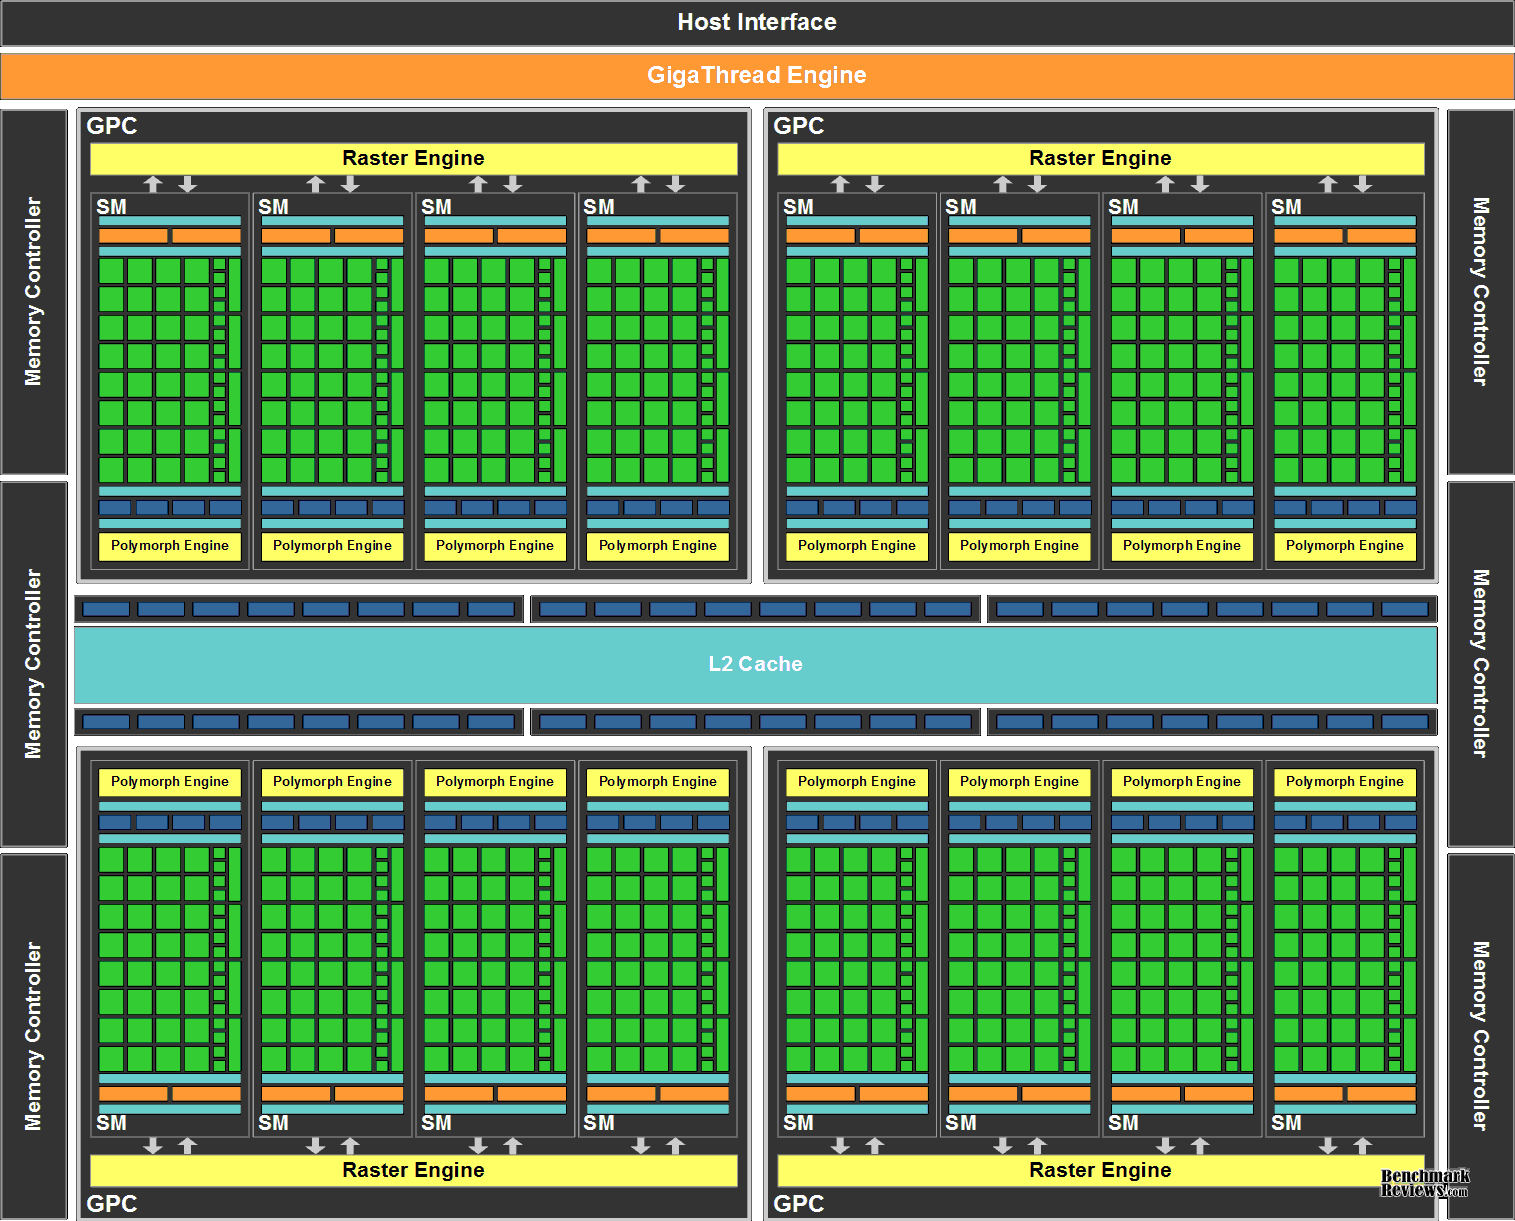
\includegraphics[width=\textwidth]{img/arq/fermi-gpu-block.pdf}
    \caption{Diagrama de bloques de GF100 Fermi. Tomado de~\cite{NvidiaFermi}.}
    \label{fermi_gpu_block}
\end{figure}

Por como funciona un pipeline gr\'afico cl\'asico, los SM se agrupan de a cuatro en GPCs (\textit{Graphics Processing Cluster}) y no interact\'ua con el modelo de c\'omputo
de CUDA.
Un esquema de esta divisi\'on global de los SM y c\'omo se comunican puede verse en la figura~\ref{fermi_gpu_block}.

%Por motivos de como funciona un pipeline gr\'afico, los SM se agrupan de 4, en un GPC (\textit{Graphics
%Processing Cluster}). Cada GPC se encarga de ejecutar los distintos pasos del pipeline gr\'afico,
%cargando a los SM con las tareas que tienen que realizar para rasterizar (es decir, convertir los
%gr\'aficos vectorialmente definidos en gr\'aficos renderizados). En aplicaciones de CUDA, estos pasos
%no importan, puesto que se trata cada SM independientemente por software.

Todos los accesos a memoria global (la memoria por fuera del procesador) se realizan a trav\'es de la cache L1 de cada SM y a trav\'es de la L2 del todo el procesador.
Esta L2 consiste de seis bancos compartidos de $128$ KB.
Estas caches se comunican de manera directa tanto con la DRAM propia de la placa como con el bus PCI Express por el cual pueden comunicarse dos placas entre s\'i, sin pasar por CPU, y son \textit{write-through}, es decir cada escritura se hace tanto en la DRAM como en la memoria cache.

%En la arquitectura Fermi, no se pueden ejecutar simult\'aneamente instrucciones de precisi\'on doble y simple y, como las de precisi\'on doble requieren ambos pipelines, suelen disminuir considerablemente el aprovechamiento de los cores.
%En la arquitectura Kepler, al usar cuatro unidades de despacho de warp, se puede elegir una mejor combinaci\'on para poder ejecutar simult\'aneamente instrucciones que no requieran usar los mismos recursos del pipeline~\cite{NvidiaKepler}.

Como estos procesadores implementan el est\'andar IEEE754-2008, cuentan con operaciones de precisi\'on simple y doble acorde al
mismo, por lo cual los c\'alculos intermedios en operaciones como FMA (\textit{Fused Multiply-Add}), que toma tres operandos y devuelve el producto de dos de ellos sumado al tercero, no pierden precisi\'on por redondeo.

%El c\'odigo escrito para CUDA se puede compilar a dos targets distintos; uno es
%el codigo binario nativo de la placa target donde se va a correr y el otro es un
%codigo intermedio, llamado c\'odigo PTX, que se JIT compila por el driver CUDA
%antes de enviar a la placa, de modo que sea portable entre placas y arquitecturas
%(retrocompatibles).

%Cuando se lanza un kernel de ejecuci\'on, este c\'odigo binario se carga en la DRAM propia
%de la placa. Este codigo va a ser ejecutado por todos los bloques que se hayan definido cuando
%se lanz\'o el kernel. El ``Thread Engine'' del GPGPU se encarga de repartir los bloques a los
%SM (Streaming Multiprocessors). Cada SM luego va a ejecutar de a grupos de 32 threads, cada uno
%de ellos corriendo sobre un SP (Streaming Processor). A traves de sus 2 o 4 unidades de dispatch de warp
%(de acuerdo a la generaci\'on de los chips), el SM puede dinamicamente cambiar el warp que se esta ejecutando en sus SP,
%escondiendo la latencia de los stalls de pipelines forzosos para la ejecucion de instrucciones de multiples clocks.
%Estos threads a su vez obtienen sus registros de un register file com\'un a todos los SP. Un scoreboard
%es mantenido por cada dispatcher de warps para poder determinar que threads estan listos para correr. En Kepler
%este scoreboard es simplificado ya que las latencias de las operaciones matem\'aticas es conocido, por
%lo cual se puede reemplazar por contadores m\'as sencillos. ~\cite{NvidiaKepler}
%Como el c\'odigo se ejecuta de manera sincr\'onica entre todos los threads del warp, las instrucciones
%condicionales proveen un problema para esta arquitectura. Como las distintas ramas del condicional
%son instrucciones excluyentes, no las deben ejecutar todos los threads simultaneamentes. El procesador
%deshabilitaba los cores que manejaban los threads de las ramas que no se ejecutaban del
%condicional~\cite{NvidiaTesla}. Para disminuir la cantidad de instrucciones de condicionales
%que se ejecutan, e cuenta con ~\cite{NvidiaFermi} predicaci\'on en todas las instrucciones de la ISA.


\section{Organizaci\'on de la memoria}

%La arquitectura CUDA esta enfocada a procesamiento de grandes cantidades de datos
%de puntos flotante. El procesador GPGPU cuenta con cientos de ALU sincronizadas
%por bloques, permitiendo un paralelismo adaptativo a distintos problemas.
%
%El procesamiento GPGPU es similar al procesamiento vectorial
%realizado por las supercomputadoras Cray y IBM que surgio en los 1960's, pero
%en vez de usar VLIW para procesamiento masivo, CUDA usa multiples hilos de ejecuci\'on
%que trabajan simultaneamente sobre los datos.
%El procesamiento consiste en un funcionamiento hibrido entre compilador y procesador. Se determina
%un conjunto de elementos a procesar y se elije de manera explicita una manera de particionar el
%problema a la hora de ser enviado para procesado a la placa.
%
%Para realizar el computo, esta arquitectura cuenta a su vez con multiples clases de memorias
%que se adaptan de maneras diferentes a los distintos procesos. Estas incluyen:

La memoria de la GPU es uno de los puntos cruciales de esta arquitectura, un esquema gr\'afico puede observarse en la figura~\ref{fig:cuda-memories}.
Esta se subdivide entre memorias on-chip y memorias on-board, de acuerdo a su ubicaci\'on y latencia de acceso, en cuatro categor\'ias distintas:

\begin{itemize}
  \item Registros
  \item Memoria local
  \item Memoria compartida
  \item Memoria global
\end{itemize}

Cada \thread{} de ejecuci\'on cuenta con una cantidad limitada de registros de punto flotante de $32$ bits con latencia de un par de ciclos de clock.
A su vez, existe una cantidad finita de registros totales que cuenta un SM (oscila entre $16535$ y $65535$ registros).
Por su baja latencia son la clase principal de almacenamiento temporal.

La memoria local es una memoria propia de cada \thread{}, y se encuentra almacenada dentro de la memoria global.
Esta memoria es definida autom\'aticamente por el compilador y sirve como \'area de almacenamiento cuando se acaban los registros: los valores anteriores se escriben a esta memoria, dejando los registros libres para nuevos valores en c\'alculos, y cuando se terminan estos c\'alculos se carga los valores originales nuevamente.
Cuenta con las mismas desventajas que la memoria global, incluyendo su tiempo de acceso.

La memoria compartida, o \textit{shared}, es una memoria que es visible para todos los \threads{} dentro de un mismo SM.
Cada \thread{} puede escribir en cualquier parte de la memoria compartida dentro de su bloque y puede ser le\'ido por cualquier otro \thread{} de este.
Es una memoria muy r\'apida, on-chip, y que tarda aproximadamente $40$ ciclos de acceso~\cite{Demystifying}.
Esta memoria es compartida con la cache L1, la cual tiene capacidad de entre $16$ KB y $64$ KB configurable por software.
Esta memoria se encuentra dividida en $32$ bancos de $2$ KB de tama\~no, permitiendo que cada uno de los $32$ \threads{} acceda independientemente a un float.
Si hubiera conflicto, los accesos a ese banco se serializar\'ian, aumentando la latencia de la llamada~\cite{farberCuda}.

La memoria global es la memoria principal fuera del chip de la GPU.
Esta es de gran tama\~no (de entre $1$ GB y $12$ GB) y es compartida por todos los SM de la GPU y los CPU que integran el sistema.
Es decir, tanto los GPU como los CPU pueden invocar las funciones de CUDA para transferir datos entre la memoria de la placa y la memoria RAM de \textit{host}.
La latencia de acceso a la memoria global es de cientos de ciclos~\cite{Demystifying}, sumamente lenta en comparaci\'on con el procesador.
La memoria global tambi\'en puede ser mapeada, o \textit{pinneada}, para que exista una copia de esa reserva tanto en la memoria en la placa como en la memoria principal del procesador. El driver de CUDA va a mantener la consistencia entre ambas de manera as\'incrona, evitando la necesidad de hacer copias de memoria expl\'icitas.
No es ilimitada la cantidad de memoria mapeada posible, por lo que es importante saber elegir qu\'e elementos se van a almacenar de esta manera.

\begin{figure}[htb]
    \centering
    \includegraphics[width=250px]{img/arq/cuda-memories_ES.pdf}
    \caption{Esquema de la jerarqu\'ia de memorias en GPU, detallando de las disponibles en cada SM, la memoria compartida (SMEN), la L2 global, la
    memoria de la placa (global) y la mapeada entre el \textit{host} y la placa de video. Tomado de~\cite{farberCuda}.}
    \label{fig:cuda-memories}
\end{figure}

Adicionalmente, la GPU cuenta con m\'ultiples niveles de memorias cache para poder aminorar el hecho de que el principal cuello de botella del c\'omputo es la latencia en los accesos a memoria global.
Estas se dividen en cuatro:

\begin{itemize}
  \item Cache L1
  \item Cache L2
  \item Cache constante
  \item Cache de textura
\end{itemize}

La cache L1 es dedicada por SM.
Esta cache fue introducida en Fermi y su dise\~no hace que tambi\'en est\'a dedicada a la memoria compartida, por lo que es posible en tiempo de ejecuci\'on darle directivas a la GPU que asigne m\'as memoria cache o m\'as memoria compartida, permitiendo a los bloques tener mayores espacios de memorias compartidas o mayores \textit{hit rates} de caches.

La cache L2 es com\'un a todos los SM de la GPU, donde, a partir de Fermi en \nvidia{}, todos los accesos de lectura y escritura a memoria global y textura pasan a trav\'es de esta~\cite{NvidiaFermi}.

La cache constante es una cache sobre la memoria global dedicada solamente a lecturas de memoria.
Esta es muy reducida (solo cuenta con $64$ KB) y est\'a optimizada para muchos accesos a la misma direcci\'on.
Cuando un \thread{} lee esta memoria, se retransmite a los dem\'as \threads{} del warp que est\'en leyendo esa misma direcci\'on, reduciendo el ancho de banda necesario.
Si, en cambio, los \threads{} leen distintas direcciones, los accesos se serializan.
Cuando hay un \emph{miss} de esta memoria, la lectura tiene el costo de una lectura de memoria global.

La cache de textura es una cache sobre la memoria global que presenta no solo localidad espacial, como la mayor\'ia de las caches de procesadores normales (es decir, la cache contiene una porci\'on consecutiva de la memoria principal), sino que se le puede agregar el concepto de dimensiones, para poder modelar datos en m\'as de una dimensi\'on.
Esto se adapta de muy bien a los problemas de gr\'aficos en 2D y 3D, y es una herramienta clave a la hora de minimizar los accesos a matrices no solo por filas sino por columnas.
Esta cache se debe definir en momento de compilaci\'on en el c\'odigo, ya que tiene l\'imites espaciales (necesarios para poder definir \'areas de memoria sobre la cual operar) y a su vez se debe acceder a los datos subyacentes a trav\'es de funciones espec\'ificas.
Una caracter\'istica adicional de esta cache es que como necesita resolver estos accesos no convencionales a la memoria, cuenta con una unidad propia de resoluci\'on de direcciones. Esta unidad tiene limitantes en cuanto a sus posibilidades, ya que no posee un ancho de banda suficiente como para resolver todos los accesos a memoria globales que podr\'ian surgir, por lo cual su uso debe ser criterioso.


\section{Esquema de paralelismo}

Al ser una arquitectura masivamente paralela desde su concepci\'on, CUDA presenta varios niveles de paralelismo, para agrupar l\'ogicamente el c\'omputo y poder dividir f\'isicamente su distribuci\'on.
Los principales son:
\begin{itemize}
  \item Bloques de \threads{}
  \item Grilla de bloques
  \item Streams
  \item M\'ultiples placas
\end{itemize}

El paralelismo a nivel de bloque instancia una cantidad de \threads{}, subdivididos l\'ogicamente en 1D, 2D o 3D.
Los \threads{} internamente se agrupan de a $32$, es decir, un \textit{warp}.
Cada uno de estos \threads{} va a contar con una manera de identificarlos un\'ivocamente: un \texttt{blockId} y, dentro de cada bloque, su propio \texttt{threadId}.
Adem\'as, van a correr simult\'aneamente en el mismo SM y van a ser puestos y sacados de ejecuci\'on de a un warp din\'amicamente por el \textit{scheduler} de hardware que cuenta cada SM.
Para compartir informaci\'on entre ellos, se puede utilizar la memoria compartida o las instrucciones de comunicaci\'on de \threads{} intrawarp (solo disponibles a partir de Kepler~\cite{NvidiaKepler}).

El paralelismo a nivel de grilla determina una matriz de bloques de ejecuci\'on que particiona el dominio del problema.
El \emph{GigaThread Scheduler} va a ejecutar cada bloque en un SM hasta el final de la ejecuci\'on de todos los \threads{} de este.
Los bloques no comparten informaci\'on entre s\'i. Por esto, no pueden ser sincronizados mediante memoria global ya que no se asegura el orden en el que ser\'an puestos a correr, y un bloque mantiene su SM ocupado hasta que termine de ejecutar, bloqueando a los dem\'as (es decir, no hay \textit{preemption} en los SM).

El paralelismo de stream es una herramienta empleada para hacer trabajos concurrentes usando una sola placa.
Esta t\'ecnica permite que m\'ultiples kernels (unidades de c\'odigo en CUDA) o copias de memoria independientes est\'en encolados, para que el driver pueda ejecutarlas simult\'aneamente si se est\'an subutilizando los recursos, de forma de minimizar tiempo ocioso del dispositivo.
Los streams permiten kernels concurrentes pero cuentan con importantes restricciones que generan sincronizaci\'on impl\'icita, lo cual hay que tener presente si se desea mantener el trabajo de forma paralela.

El paralelismo a nivel de placa consiste en poder distribuir la carga del problema entre distintas GPUs dispuestas en un mismo sistema compartiendo una memoria RAM com\'un como si fuera un software multithreaded tradicional.
CUDA no cuenta con un modelo impl\'icito de paralelismo entre distintas placas, pero es posible hacerlo manualmente eligiendo de manera expl\'icita qu\'e dispositivo usar.
Las placas se pueden comunicar as\'incronamente entre s\'i, tanto accediendo a las memorias globales de cada una como ejecutando c\'odigo remotamente.
En las versiones modernas del driver de CUDA, tambi\'en pueden comunicarse directamente las placas entre s\'i a trav\'es de la red, permitiendo escalar multinodo f\'acilmente en un cluster de c\'omputo~\cite{farberCuda}.

\section{Diferencias entre Tesla, Fermi, Kepler}

Hasta ahora se describi\'o la arquitectura vista desde el punto de vista Fermi, que es la segunda arquitectura GPGPU dise\~nada por \nvidia{}.
Fermi es la evoluci\'on de Tesla, construida para desacoplar a\'un m\'as los conceptos de procesamiento gr\'afico de modo de lograr un procesador m\'as escalable y de prop\'osito general.
La arquitectura sucesora a Fermi es Kepler, presentada en el 2012, con las metas de disminuir el consumo y aumentar la potencia de c\'alculo~\cite{NvidiaKepler}.

\begin{table}[h]
  \begin{tabular}{@{}llll@{}}
  \toprule
  Caracter\'isticas        & Tesla (GT200)   & Fermi (GF100)   & Kepler (GK110)   \\ \midrule
  A\~no introducci\'on     & 2006            & 2010            & 2012             \\
  Transistores             & 1400 millones   & 3000 millones   & 3500 millones    \\
  Tecnolog\'ia fabricaci\'on & 65 nm           & 40 nm           & 28 nm            \\
  SMs                      & 30              & 16              & 15               \\
  SP / SM                  & 8               & 32              & 192              \\
  Cach\'e L1               & -               & 16 - 48 KB       & 16 - 32 - 48 KB   \\
  Cach\'e L2               & -               & 768 KB           & 1536 KB           \\
  Memoria Shared/SM      & 16 KB            & 16 - 48 KB       & 16 - 32 - 48 KB   \\
  Registros/Thread         & 63              & 63              & 255              \\
  Pico Precisi\'on Simple    & 240 MAD / clock & 512 FMA / clock & 2880 FMA / clock \\
  Pico GFLOPS Simple       & 933             & 1345            & 3977             \\
  GFLOPS/Watt              & $3.95$            & $5.38$            & $15.9$             \\ \bottomrule
  \end{tabular}
\caption{Tabla comparativa de las caracter\'isticas m\'as prominentes de las tres arquitecturas de CUDA.}
\label{tab:CudaGenerations}
\end{table}

En la tabla \ref{tab:CudaGenerations} se ve una comparaci\'on de las recursos que est\'an m\'as directamente relacionados a la \performance{} de un dispositivo GPU.
Se puede apreciar el crecimiento notable del poder de c\'omputo debido a las tecnolog\'ias de fabricaci\'on, que permitieron aumentar la cantidad de transistores por unidad de superficie.
Tambi\'en se puede comprobar que, a diferencia de los CPU, las arquitecturas GPGPU decidieron utilizar esos nuevos transistores disponibles para m\'as n\'ucleos de procesamiento, en vez
de dedicarlas a aumentar las memorias cache, que crecieron m\'inimamente (comparando contra las caches de CPU).

Una de las diferencias m\'as notorias entre Tesla y Fermi es la presencia de FMA contra el MAD (\textit{Multiply - Add}).
El MAD realiza la multiplicaci\'on y la acumulaci\'on en dos pasos, pero m\'as r\'apidos que hacerlos independientemente por tener hardware dedicado.
Debido a que debe redondear entre los pasos, pierde precisi\'on y no respeta completamente el est\'andar IEEE754-2008.
El FMA, en cambio, lo hace en una sola operaci\'on, y sin redondeos intermedios.

La m\'etrica usada por \nvidia{} para publicitar la \performance{} de estos dispositivos y poder compararlos entre s\'i, y contra CPU, son los GFLOPS.
Esta unidad mide cuantas operaciones de punto flotante de precisi\'on simple se pueden realizar por segundo.
Los GFLOPs son utilizados tambi\'en por los clusters en el ranking TOP500, donde se ordenan de acuerdo a la \performance{} medida usando un software estandarizado, \texttt{LINPACK}.
No solo es notable como se cuadruplic\'o la \performance{} (te\'orica) en solamente seis a\~nos, sino que a\'un m\'as importante es como mejor\'o la \performance{} por Watt.
Esto tambi\'en se ve en que Kepler tiene menos SM que Fermi o Tesla, pero son mucho m\'as poderosos y eficientes.
La tecnolog\'ia de fabricaci\'on ha ayudado a la disminuci\'on del consumo, un problema que acechaba a los dise\~nos Fermi, ya que sus consumos superiores a 200W por dispositivo los hac\'ian muy dif\'iciles de refrigerar incluso en clusters de HPC.
Se puede apreciar entonces la estrategia de mercado de \nvidia{} de introducirse en las supercomputadoras de todo el mundo, donde el consumo y la refrigeraci\'on son factores limitantes (mucho m\'as a\'un que, por ejemplo, en computadoras de escritorio)~\cite{HennessyPatterson}.

\section{CUDA, Herramientas de desarrollo, profiling, exploraci\'on}

Para soportar una arquitectura masivamente paralela, se debe usar una ISA (\textit{Instruction Set Architecture}) dise\~nada especialmente para el problema.
En el caso de CUDA, esta ISA se denominada PTX y debe poder soportar conceptos fundamentales del c\'omputo GPGPU: grandes cantidades de registros, operaciones en punto flotante de precisi\'on simple y doble, y FMA~(fused multiply-add).
Adem\'as, el c\'odigo compilado para GPU debe ser agn\'ostico al dispositivo que lo va a correr, por lo cual la paralelizaci\'on no debe estar demasiado atada a este, sino que el dispatching lo debe poder determinar el driver de la placa en tiempo de ejecuci\'on.
Un \'ultimo requerimiento clave de esta ISA es que debe soportar hacer ajustes manuales, para poder construir partes claves de ciertas bibliotecas frecuentemente usadas (como las
rutinas de BLAS de \'algebra lineal)~\cite{NvidiaFermi}.

El lenguaje CUDA es una extensi\'on de C++, con ciertas caracter\'isticas agregadas para poder expresar la subdivisi\'on de las rutinas en \threads{} y bloques, junto con mecanismos para especificar qu\'e variables y funciones van a ejecutarse en la GPU y en el CPU.
Una caracter\'istica de CUDA es que todas las llamadas a los kernels de ejecuci\'on son asincr\'onicas, por lo que es relativamente sencillo solapar c\'odigo en GPU y CPU.
A su vez se cuenta con m\'ultiples funciones opcionales, con distinta granularidad, que permiten esperar a que todas las llamadas as\'incronas a GPU finalicen, agregando determinismo
en forma de barreras de sincronizaci\'on al lenguaje.

El c\'odigo CUDA compila usando \texttt{nvcc}, una variante del \texttt{GNU gcc} que se encarga de generar el c\'odigo PTX para las funciones que se van a ejecutar en las GPU.
Este c\'odigo objeto despu\'es se adosa normalmente con el resto del c\'odigo que corre en CPU y se genera un binario ejecutable.

\nvidia{}, adem\'as, provee herramientas de profiling para explorar c\'omo se est\'an utilizando los recursos durante la ejecuci\'on.
\'Estas son esenciales para optimizar, puesto que los limitantes de GPU son sumamente distintos a los de CPU, presentando dificultades conceptuales incluso para programadores experimentados.
Las herramientas de profiling no solo muestran \emph{runtime}, sino que sirven para ver d\'onde hay accesos a memoria excesivos, puntos de sincronizaci\'on costosos, limitantes en los registros y c\'omo se superponen las llamadas asincr\'onicas.

El uso de todas estas herramientas fue vital en este trabajo para poder entender c\'omo funciona la arquitectura en detalle, c\'omo medir \performance{} y utilizaci\'on, y c\'omo los cambios realizados impactaron en las distintas generaciones de dispositivos.

\section{Requerimientos de un problema para GPGPU}

Dada la organizaci\'on de un procesador GPU, un problema debe exhibir al menos las siguientes caracter\'isticas para que tenga potencialidad para poder aprovechar las caracter\'isticas y recursos disponibles en esta arquitectura:

\begin{enumerate}
  \item \label{req:paralelo} El problema debe tener una gran parte paralelizable.
  \item \label{req:float} El problema debe consistir, mayormente, de operaciones num\'ericas.
  \item \label{req:matrix} El problema debe poder ser modelado, en su mayor parte, utilizando arreglos o matrices.
  \item \label{req:transf} El tiempo de c\'omputo debe ser muy superior al tiempo de transferencia de datos.
\end{enumerate}

El \'item \ref{req:paralelo} se refiere a que debe existir alguna forma de partir el problema en subproblemas que puedan realizarse simult\'aneamente, sin que haya dependencias de
resultados entre s\'i.
Si el problema requiere partes seriales, lo ideal es que se las pueda dividir en partes independientes que sean etapas de una cadena de procesos, donde cada una de \'estas exhiban caracter\'isticas fuertemente paralelas.
Como las arquitecturas masivamente paralelas tienen como desventaja una menor eficiencia por n\'ucleo, si el problema no se puede dividir para maximizar la ocupaci\'on de todos los procesadores disponibles, va a resultar muy dif\'icil superar en eficiencia a los procesadores seriales.

El ítem~\ref{req:float} habla acerca de que el m\'etodo de resoluci\'on de los problemas debe provenir de una aplicaci\'on num\'erica o de gran carga aritm\'etica.
El set de instrucciones de las arquitecturas GPGPU est\'an fuertemente influenciados por las aplicaciones 3D que las impulsaron en un principio.
\'Estas consisten mayormente de transformaciones de \'algebra lineal para modelar iluminaci\'on, hacer renders o mover puntos de vistas.
Todos estos problemas son inherentemente de punto flotante, por lo cual el set de instrucciones, las ALUs internas y los registros est\'an optimizados para este caso de uso.

El ítem \ref{req:matrix} menciona que los problemas que mejor se pueden tratar en esta arquitectura se pueden representar como operaciones entre arreglos o matrices de dos, tres o cuatro dimensiones.
Las estructuras de datos no secuenciales en memoria incurren en m\'ultiples accesos a memoria para recorrerlas y, en las arquitecturas GPGPU, generan un gran cuello de botella.
Adem\'as, suelen ser dif\'iciles de paralelizar en m\'ultiples subproblemas.
Tener como par\'ametros de entrada matrices o arreglos que se puedan partir f\'acilmente producen en overheads m\'inimos de c\'omputo y permiten aprovechar mejor las memorias caches y las herramientas de prefetching que brinda el hardware.

El \'item \ref{req:transf} ataca uno de los puntos cr\'iticos de esta arquitectura.
Para poder operar con datos, se requiere que est\'en en la memoria de la placa, no en la memoria de prop\'osito general de la computadora.
Se debe, entonces, hacer copias expl\'icitas entre las dos memorias, ya que ambas tienen espacios de direcciones independientes.
Esta copia se realiza a trav\'es de buses que, a pesar de tener un gran \emph{throughput}, tambi\'en tienen una gran latencia (del orden de milisegundos).
Por lo tanto, para minimizar el tiempo de ejecuci\'on de un programa usando GPGPUs, se debe considerar tambi\'en el tiempo de transferencia de datos a la hora de determinar si el beneficio de computar en menor tiempo lo justifica.
Las nuevas versiones de CUDA buscan brindar nuevas herramientas para simplificar este requerimiento, proveyendo espacio de direccionamiento \'unico y memoria unificada~\cite{farberCuda}, pero siguen siendo copias de memoria a trav\'es de los buses (aunque asincr\'onicas).

Estas caracter\'isticas limitan enormemente la clase de problemas que una GPGPU puede afrontar, y suelen ser una buena heur\'istica para determinar de antemano si vale la pena
invertir el tiempo necesario para la implementaci\'on y ajuste fino.

\section{Diferencia entre CPU y GPU - Procesadores especulativos}

Hasta ahora, solo se consideraron a los GPUs de forma aislada, observando las prestaciones del hardware y una aproximaci\'on a la manera en que se escriben los programas para esta arquitectura.
La esencia de GPGPU se puede apreciar mejor compar\'andola contra los motivos de la evoluci\'on de CPU, y los problemas que se fueron enfrentando los dise\~nos siguiendo la historia de los componentes que fueron apareciendo en estos.
% Esto se mostr\'o en la tabla \ref{tbl:historia-cpu} (p\'agina~\pageref{tbl:historia-cpu}), que detalla algunos de los eventos m\'as importantes que aceleraron
% la \performance{} de los CPU.

Lo clave es observar el siguiente patr\'on: \emph{``no desechar algo que pudi\'eramos necesitar pronto''}, \emph{``intentar predecir el futuro de los condicionales''}, \emph{``intentar correr m\'ultiples instrucciones a la vez porque puede llegar a bloquear en alguna de ellas''}.

Todos estos problemas han convertido al CPU en un dispositivo que gira alrededor de la especulaci\'on, de los valores futuros que pueden tener las ejecuciones, del probable reutilizaci\'on de datos.
En un CPU moderno (por ej. Intel Xeon E7-8800~\cite{XeonE78800Spec}) las unidades que verdaderamente realizan las operaciones l\'ogico-aritm\'eticas (las ALU) son muy pocas en comparaci\'on con la cantidad utilizadas para las operaciones de soporte.

En contraste, los dispositivos GPU son verdaderos procesadores de c\'omputo masivo.
Est\'an dise\~nadas para resolver constantemente operaciones muy bien definidas (instrucciones de punto flotante en su mayor\'ia).
Comparativamente con un CPU, las ALU de las GPU son bastante pobres y lentas.
No funcionan a las mismas velocidades de clock (rara vez superan $1.1$ GHz) y sus SP deben estar sincronizados entre s\'i.
Pero la gran ventaja esta en la cantidad.

Un CPU cuenta con pocas ALU por core, dependiendo de la cantidad de cores y del tama\~no de sus operaciones SIMD (alrededor de $16$ cores por \emph{die} de x86 es el tope de l\'inea ofrecido actualmente, procesando de a $32$ bytes simult\'aneamente).
Un GPU cuenta con miles de ALUs en total (m\'as de $2500$ CUDA cores en una Tesla K20~\cite{NvidiaKeplerDatasheet}).
El dise\~no de esta arquitectura concibe la escalabilidad cuantitativa de las unidades de c\'omputo como la caracter\'istica esencial a tener, tanto por su \'enfasis fundamental, las aplicaciones gr\'aficas, como para su aspecto de coprocesador num\'erico de prop\'osito general.

Por contrapartida, los GPUs disponen de pocas unidades de soporte del procesamiento.
\'Estos no disponen de pipelines especulativos, el tama\~no de las caches est\'an a \'ordenes de magnitud de las de CPU, la latencia a las memorias principales de la GPU est\'an a centenas de clocks de distancia, etc.
La arquitectura supone que siempre va a tener m\'as trabajo disponible para realizar, por lo cual en vez de intentar solucionar las falencias de un grupo de \threads{}, directamente
pone al grupo en espera para m\'as adelante y contin\'ua procesando otro warp de \threads{}.
Se puede notar que durante del dise\~no de la arquitectura CUDA, buscaron resolver el problema del c\'omputo masivo pensando en hacer m\'as cuentas a la vez y recalcular datos, si fuera necesario.
Esto es una marcada diferencia con respecto a los CPU, que est\'an pensados en rehacer el menor trabajo posible e intentar mantener todos los datos que pueda en las memorias caches masivas.

Nuevamente, en este punto se puede apreciar el legado hist\'orico de los CPU.
Al tener que poder soportar cualquier aplicaci\'on, no pueden avocarse de lleno a una sola problem\'atica.
Para las arquitecturas GPGPU, el hecho de no tener que dise\~nar un procesador de prop\'osito general compatible con versiones anteriores, permiti\'o un cambio radical a la hora de concebir una arquitectura de gran throughput auxiliar al procesador, no reemplaz\'andolo sino m\'as bien adicionando poder de c\'omputo~\cite{GlaskowskyFermi}.

Las arquitecturas Tesla, Fermi y Kepler conciben el dise\~no de un procesador de alto desempe\~no.
Su meta principal es poder soportar grandes cantidades de paralelismo, mediante el uso de procesadores sim\'etricos, pero tomando la fuerte restricci\'on de \textsl{``no siempre tiene que andar bien''}.
Es decir, los dise\~nadores suponen que el c\'odigo que van a ejecutar esta bien adaptado a la arquitectura y no disponen casi de mecanismos en el procesador para dar optimizaciones post-compilaci\'on.
Relajar esta restricci\'on permite romper con el modelo de c\'omputo de CPU y definir nuevas estrategias de paralelismo, que no siempre se adaptan bien a todos los problemas, pero para el subconjunto de los desaf\'ios que se presentan en el \'area de HPC y de v\'ideo juegos han probado ser un cambio paradigm\'atico.

\section{Idoneidad para la tarea}

El método de dinámica molecular tratado en este trabajo es un problema que implica una gran cantidad de operaciones matemáticas de gran volumen de cálculos e independientes entre si.
El cálculo de fuerzas, la suma de todas las fuerzas parciales y la actualización de coordenadas son todos cálculos que se deben resolver para todas las partículas de forma individual. 
Esto implica una gran cantidad de cálculos pero además una gran cantidad de datos que deben ser actualizados en cada paso de la simulación.
En particular, la gran cantidad de accesos necesarios para actualizar constantemente los datos asociados a cada partícula constituye un cuello de botella en este tipo de aplicaciones.

Dadas las caracter\'isticas de contar con un fuerte nivel de paralelismo y de ser operaciones mayormente de punto flotante, hace ya algún tiempo 
las arquitecturas GPU se convirtieron en estándar para la aplicación de métodos de DM, tal como se vió en el capítulo 1.

% De todas formas, aún queda mucho por avanzar. 


% se determin\'o que el uso de GPGPU para este problema era promisorio, en comparaci\'on con arquitecturas de prop\'osito general con menos poder de c\'omputo. 


% 
% El problema de QM/MM enfrentado en este trabajo cuenta con m\'ultiples operaciones matem\'aticas de gran volumen de c\'alculos.
% En particular, las operaciones matriciales constituyen los principales cuellos de botella en esta aplicaci\'on.
% Estas operaciones se realizan para varios grupos dentro de una grilla de integraci\'on (ecuaci\'on~\ref{eq:xc}), los cuales se pueden realizar de manera independiente (y por lo tanto en paralelo).
% 
% Para obtener los valores num\'ericos de densidad buscados en los puntos, se deben obtener las derivadas primeras y segundas, lo cual implica hacer m\'ultiples operaciones de multiplicaci\'on matricial.
% Este tipo de problemas est\'a estudiado fuertemente en la literatura debido a la multiplicidad de aplicaciones de diferentes campos que requieren de operaciones de \'algebra lineal.
% 
% En nuestro caso, para un sistema se requieren miles de estas multiplicaciones entre matrices, algunas con matrices de m\'as de $500^2$ elementos.
% Como LIO es un proyecto de resoluci\'on num\'erica de QM/MM, los problemas enfrentados son casi, en su totalidad, operaciones de punto flotante.
% Luego, dadas las caracter\'isticas de contar con un fuerte nivel de paralelismo en los cuellos de botella y de ser operaciones mayormente de punto flotante, 
% se determin\'o que el uso de GPGPU para este problema era promisorio, en comparaci\'on con arquitecturas de prop\'osito general con menos poder de c\'omputo. 
% La exploraci\'on original de esta arquitectura trajo buenos resultados, por lo que se prosigui\'o su an\'alisis como un camino prometedor~\cite{TesisNitsche}.




\chapter{Algoritmos}


En este capítulo, los conceptos del m\'etodo de dinámica molecular presentados en la introducción son explicados en términos del algoritmo que los representa,
haciendo énfasis en el paralelismo intrínseco que poseen, intentando abstraerse de cualquier implementación.

En la primera sección se describen los conceptos del algoritmo base, describiendo todos los pasos de éste, en particular los detalles que no fueron abordados en la introducción. 

En las siguientes secciones del capítulo, se explican las modificaciones que este trabajo introduce y las propiedades que se deben tener en cuenta para implementarlas utilizando arquitecturas paralelas.

% Es importante destacar que las adaptaciones que se plantean y analizan en este trabajo constituyen una modificación puntual para realizar el calculo del potencial de Lennard-Jones y, por lo tanto, 
% tienen la capacidad de ser incluidas directamente en cualquier implementación existente y combinadas junto con cualquier otro método de optimización.
% Por otro lado, como se vió en el capitulo 1, existen pocas variantes para optimizar el cálculo de este potencial de no-unión y, dado que comprende el mayor aporte al costo computacional del método, 
% estas modificaciones pueden tener un gran impacto en la .


%Dado que el aporte a las interacciones que nos interesa es el correspondiente al potencial de L-J , este es el unico que se va a considerar. 
%Es decir, el campo de fuerzas estará definido exclusivamente por el potencial de Lennard-Jones que modela interacciones de no-unión. 
%De esta forma, el sistema evoluciona en el tiempo a partir de las velocidades iniciales de las particulas y las fuerzas que se derivan de este potencial, unicamente. 
% Sin embargo, usando el modelo de interacción resultante no será posible simular (de forma correcta) sistemas moleculares que incluyan enlaces químicos, ya que estos no estarán correctamente modelados por el campo de fuerzas. 
% El objetivo de esto es, en primer lugar, facilitar la implementacion de modificaciones/optimizaciones en el algoritmo relacionadas con el calculo del potencial de L-J.
% En segundo lugar, utilizando una implementacion propia se puede evaluar las ventajas y desventajas del uso de una tabla numerica de forma independiente a cualquier otra implementacion existente. 
% Se podrá verificar facilmente que las variaciones en el tiempo y en la precision de los resultados son producto exclusivo de las modificaciones implementadas en cada paso.




\section{Esquema general del algoritmo}

El algoritmo base sigue la especificación que se detalló en el capítulo 1(figura \ref{esquemaMD}). 

El primer paso de la iteración implica calcular la fuerza que actúa sobre cada partícula. 
El cálculo de la fuerza entre \textbf{cada par} de partículas responde a la siguiente ecuación: \begin{equation} \label{fuerza}\vec{F}(r)=\dfrac{\partial U(r)}{ \partial r}\end{equation}
  
Por lo tanto, para obtener el valor de la fuerza puntual entre las partículas, primero debemos conocer el valor de \textit{r}, es decir, la distancia entre cada par de estas. 
El cálculo necesario para obtener estas distancias es simplemente la resta entre los componentes de las coordenadas de cada partícula, lo que hace que sea fácilmente paralelizable 
ya que las posiciones son totalmente independientes entre si. 

En el caso que se estén utilizando condiciones periódicas de borde, la distancia entre cada par de partículas se debe calcular sólo para las imágenes mas cercanas.

A partir de las distancias entre las partículas, la ecuación \ref{fuerza} permite obtener la fuerza resultante de la interacción entre ellas, conociendo la función potencial.
Este valor corresponde a la fuerza en la dirección de $\vec{r}$, es decir, la dirección del vector distancia. 
Para poder obtener la suma total de las fuerzas que actúan sobre una partícula, como resultado de interacciones con todos los demás elementos del sistema,
es necesario sumar todos los aportes. Esto implica sumar fuerzas con distintas direcciones(distintos vectores distancia), lo que se traduce en una suma de los componentes \textit{x,y,z} de los distintos vectores. 
Por lo tanto, el cálculo de la fuerza total que actúa sobre una partícula se divide en tres pasos:

\begin{itemize}
\item En un primer paso se calcula el valor de la fuerza entre cada par de partículas de acuerdo a la ecuación \ref{fuerza}, desarrollando la derivada para el potencial de Lennard-Jones:

\begin{equation} 
  \vec{F}(r)=\dfrac{\partial(U(r)) }{ \partial r}  =  24\epsilon \bigg(\dfrac{{\sigma}^{6}}{{r}^{7}} - \dfrac{2{\sigma}^{12}} {{r}^{13}}\bigg)
\end{equation}


\item En un segundo paso se descompone esta fuerza en sus 3 componentes \textit{x,y,z}: \begin{equation}                                                                                
F_i=\vec{F}(r)\dfrac{\partial r}{\partial i}  \hspace{30pt} \textit{para i= x,y,z}
                                                                                 \end{equation}

\item Por último se realiza la suma de los componentes para todas las fuerzas que actúan sobre una partícula \textit{j}: 
\begin{equation}
F^j_i=\sum F_i	\hspace{30pt} \textit{para i= x,y,z}
\end{equation}

\end{itemize}



% CALCULO DE LA ACELERACION/CAMBIO EN LA VELOCIDAD
Una vez obtenida la fuerza que actúa sobre cada partícula(componetes \textit{x,y,z}), se puede calcular la aceleración(\textit{a}=cambio en la velocidad) resultante de ésta,
y actualizar la velocidad de la partícula de acuerdo al cambio ocurrido.
La velocidad estará dada por:
 \begin{equation} 
    v(t+dt)= v(t) + a\times dt =  v(t) + \bigg(\frac{F}{masa}\bigg)\times dt
% velocity[i] = Vt + ( (force[i]*dtx) / m[type] );
 \end{equation}

Nuevamente, la velocidad depende de variables individuales de cada elemento (velocidad anterior, fuerza y masa) y el cálculo es totalmente independiente para las distintas partículas.  




% PASO DE ACTUALIZACION DE CORDENADA
El proceso de actualización de coordenadas deberá calcular para cada partícula su nueva posición, la cual estará dada en función de las coordenadas anteriores, la velocidad que se calculó previamente en la iteración y el \textit{step} en el tiempo(\textit{dt}). 
La ecuación que se debe resolver en este paso es:
\begin{equation} 
    Pos_x(t+dt)= Pos_x(t) + (v_x \times dt)
% positions[i] = positions[i] + (velocity[i] * dtx);
\end{equation}

Claramente, este cálculo es totalmente independiente entre las partículas y por lo tanto puede paralelizarse por completo.

El tiempo se ejecución para esta serie de pasos limita su aplicación sobre algunos problemas biológicos de interés, no sólo por la complejidad intrínseca del algoritmo ($N^2$), sino porque, aún en arquitecturas altamente paralelas como
las GPUs (cuyo número de unidades de cálculo ha crecido exponencialmente), no es tan simple obtener el máximo de performance teórico de la arquitectura. 
Estas limitaciones para poder realizar todos los cálculos con la máxima eficiencia se deben, principalmente, a la baja performance en los accesos a memoria. 
Es necesario, entonces, realizar aproximaciones extra para acercarse a este límite.


\section{Cálculo usando tablas de valores del potencial }


Basándose en la forma funcional del potencial mostrada en el capítulo 1(figura \ref{lennardimage}), es razonable pensar que, utilizando una tabla que contenga los resultados de esta ecuación en un rango definido de valores de \textit{r}, y, 
aún sin tener ésta un tamaño excesivo, será posible obtener una estimación bastante aproximada de la interacción entre dos partículas. 

Utilizando esta tabla, para obtener el valor de la energía potencial de interacción entre un par de partículas simplemente se debe recuperar el resultado asociado a la distancia(\textit{r}) entre estas(o el valor tabulado más cercano).
% Esta propiedad se deriva directamente de las características de la función y es independiente del esquema de dinámica molecular.


% Teniendo este tipo de valores almacenados es posible utilizarlos para calcular tanto las fuerzas resultantes (necesarias para la evolucion de la simulacion) como el valor de la enegia potencial total, el cual puede ser requerido por el usuario como resultado de la simulacion.
Para insertar este método dentro del algoritmo de dinámica molecular debemos analizar primero la forma de obtener, a partir de éste, el valor de la fuerza para la distancia correspondiente.
% En la sección anterior se mostró como el algoritmo utiliza este potencial para obtener la interacción entre cada par de particulas y derivar la fuerza resultante. 
Como se mostró previamente, conociendo la derivada del potencial en función de la distancia entre los átomos, la fuerza se obtiene a partir de la ecuación \ref{fuerza}.

Implementando una tabla que contenga valores del potencial, se puede estimar el valor de la derivada mediante la técnica de derivación numérica. 
Para esto se obtienen primero dos valores de potencial a partir de la tabla, correspondientes a distancias de $r\pm h$ (donde h es un valor discreto definido en base a la forma funcional y el tamaño total de la tabla).
La aproximación de la derivada se calcula entonces como:

\begin{equation}
 U'(r) \approx \frac{U(r+h)-U(r-h)}{2h}
\end{equation}

Utilizando estas aproximaciones, aplicadas dentro de un esquema de dinámica molecular, sería posible simplificar considerablemente el paso correspondiente al cálculo de las fuerzas resultantes entre las partículas.

La aproximación del valor de la derivada por el método de derivación numérica entrega resultados aceptables con un determinado error. 
El uso de valores tabulados tiene, a su vez, un error asociado que depende principalmente del tamaño de la tabla.
La utilización del método junto con el esquema de valores tabulados implica, entonces, una doble fuente de error. 

El algoritmo de dinámica molecular utiliza la fuerza para modificar la posición de las partículas influyendo, a su vez, sobre el valor que tendrá el potencial en la próxima iteración. 
De esta forma, los errores resultantes del método serán propagados a lo largo de una simulación que, normalmente, involucra miles de pasos.
Una parte importante de aplicar esta aproximación será, entonces, asegurar la correctitud numérica de los resultados, 
principalmente la estabilidad a lo largo de una simulación que involucra una gran cantidad de pasos y que genera la propagación de los errores.


Como se vió previamente, la ecuación del potencial de Lennard-Jones (ecuación \ref{lennardEquation}) depende directamente de \textit{r} y de los valores de $\epsilon$ y $\sigma$ de ambas partículas.
Para implementar este método se necesitará, entonces, una tabla con tres dimensiones. En una dimensión el valor del potencial variará en función de \textit{r}.
Las otras dos dimensiones representan una matriz que contiene todas las combinaciones de pares $\epsilon$-$\sigma$.

Una ventaja adicional de tener tabulados los valores del potencial es que permite calcular muy fácilmente el valor de la energía potencial total asociada a una conformación puntual del sistema.
Para esto solo se debe recuperar los valores de la tabla asociados a cada interacción encontrada en el sistema y luego obtener la suma de estos.
Si bien la salida principal del método es la trayectoria que sigue cada partícula, suele adjuntarse, además, el valor de $E_tot$ asociado a la conformación del sistema cada cierta cantidad de pasos. 
Este valor es utilizado durante el proceso de análisis posterior que se realiza sobre los resultados.


\section{Valores tabulados de la derivada}

Como se mencionó en el capítulo 1, el método de dinámica molecular está centrado en calcular la evolución del sistema a lo largo del tiempo, es decir, las posiciones en el espacio de todos sus elementos describiendo una trayectoria. 
Además de ser la base de la simulación, y que por lo tanto necesita ser resuelta para guiar la evolución del sistema, la trayectoria resultante es utilizada luego para obtener las conclusiones químicas relevantes del proceso analizado. 
En este contexto, el potencial de L-J es utilizado únicamente para obtener, a través de su derivada, la fuerza generada mediante las interacciones entre partículas. 

Se podría pensar que una forma mas eficiente de aprovechar el sistema de valores tabulados sería mantener en una tabla los valores de la derivada, en lugar de almacenar valores resultantes del potencial. 
De esta forma, para obtener la fuerza correspondiente, se busca el valor en la tabla asociado a la distancia \textit{r} entre las partículas (o el valor tabulado mas cercano). 

% ya que es la base de la simulación, se debe obtener siempre, y a partir de ella se realizan luego las conclusiones químicas relevantes.
% Para poder obtener esta trayectoria, el potencial de L-J s
% Dado que el valor mas importante que se obtiene a partir del potencial de L-J es la fuerza resultante de la interacción, 
% se podría pensar que sería mas conveniente, en lugar de tabular valores del potencial,

Las ventajas de esta nueva aproximación son claras: se reduce el error, ya que los valores tabulados fueron calculado directamente mediante la ecuación asociada a la derivada, 
y se reduce la complejidad del acceso a memoria, ya que sólo se requiere leer un valor de la tabla para obtener el resultado de la derivación.


\section{Posibilidades de implementación}

Se debe tener en cuenta que la implementación de un sistema de valores tabulares requerirá una carga extra de acceso a memoria, por lo tanto, es necesaro analizar alternativas posibles para que estos accesos se logren de manera eficiente.
La forma de implementar y utilizar las tablas debería ser, de todas formas, bastante directa y simple, pero es necesario hacer un análisis exhaustivo de los posibles errores en los resultados,
además de evaluar objetivamente las ventajas que provee en términos de eficiencia.

Es importante aclarar que las modificaciones planteadas apuntan a optimizar la etapa correspondiente al cálculo de fuerzas, el contexto de este paso en el algoritmo se mantiene sin modificaciones.
Por otro lado, aún cuando el objetivo de este trabajo se centra en estudiar la eficienca de las implementaciones sobre GPUs, la solución aqui planteada puede ser implementada en distintas arquitecturas.




\chapter{Implementaciones}

\begin{comment}
Aca describo el kernel y aspectos relevantes de las versiones implementadas:
-que variables tengo que tener en cuenta en las implementaciones(por ej. el tamaño de la tabla,el rango, etc)
-que resultados espero!
-como afecta la periodicidad. la describo aca o en la parte de resultados??
-como afecta el tamaño de los bloques
\end{comment}

En este capítulo se describen los kernels implementados, incluyendo las variantes evaluadas. Además, se detalla cómo se tuvieron en cuenta los aspectos de performance expuestos en el capítulo 2.



\section{Consideraciones previas}

Una de las primeras decisiones que se deben considerar es la precisión que se utilizará para realizar los cálculos y acumular resultados. Dadas las caracterísiticas de la arquitectura GPU, esta decisión afectará la eficiencia de cualquier cálculo a realizar y por lo tanto es uno de los factores mas importantes a analizar.

Si bien es un factor importante, este ya ha sido estudiado usando otras implementaciones del método.  En particular, se ha estudiado usando Amber\cite{le2013spfp}. El trabajo mencionado analiza un esquema mixto que implica almacenar los calculos de fuerzas entre particulas utilizando precisión simple y acumular en variables de precisión doble la suma de todos los aportes que componen la fuerza sobre una partícula. Asumiendo los resultados en performance y correctitud encontrados en Amber y,
dado que es el software con el cual evaluaremos luego la calidad numérica lograda, utilizaremos, entonces, un esquema similar de precisión para nuestra implementación.



\section{Esquema general de la implementación sobre GPU}
El esquema general utilizado para implementar el algoritmo sobre GPU es el explicado en \cite{friedrichs2009accelerating}. Sin embargo, en el trabajo mencionado, el potencial incluye componentes de interacción de unión entre partículas, 
por lo que los calculos requeridos son algo distintos. En esta sección se explica, entonces, cuales son las variantes que utilizamos para realizar cada paso.

Para el primer paso de calculo de distancias entre partículas, la implementación es bastante directa. La granularidad usada es de 1 thread por cada par de partículas y se usaron tamaños de bloques fijos dd 1024x1.
Usando este esquema, con cualquier placa actual es posible lanzar en paralelo el calculo de todas las distancias para sistemas de hasta Xxx partículas. Teniendo en cuenta  que  el cálculo a realizar es muy simple, no presenta posibilidades de divergencia y dado el esquema de acceso a memoria, el kernel hace un uso óptimo de los recursos.

El paso correspondiente al calculo de las fuerzas entre particulas es quizas el mas complicado de implementar, y el numero de implementaciones existentes en la literatura es muy diversa, principalmente debido a que los calculos a realizar dependen de las interacciones que se estan utilizando y estás dan lugar a una gran variedad de posibles optimizaciones
\cite{friedrichs2009accelerating}\cite{gotz2012routine}\cite{salomon2013routine}
(citar los papers de amber y el de Accelerating Molecular Dynamic Simulation on Graphics Processing Units)

En el caso de interacciones non-bond, como las que se analizan en nuestro trabajo, la principal optimizacion deriva de la propiedad simetrica que presenta el potencial de interaccion, y por lo tanto la fuerza resultante, son simetricas

En nuestra implementación, esta parte es central ya que da lugar luego a diversas modificaciones. El presente trabajo, entonces, intenta seguir una implementacion estandar de forma tal que las modificaciones evaluadas tengan un carácter mas general y no dependan de ninguna

Para hacer uso de la propiedad de simetria, entonces, el calculo de la fuerza resultante de la interaccion solo se realiza sobre N2/2 pares, y el resto se deriva negando este valor.

Para descomponer las componentes el cálculo se realiza usando un thread por cada par de partículas.
Y para hacer la suma de la fuerza resultante, este se hace directamente sumando todos los valores de una fila. El acceso en este caso es coalescente ????? Y si hago una reducción ???

Los pasos siguientes son, bastante directos.
La aceleración se calcula en base a la fuerza resultante usando un thread por cada partícula.
La actualización de coordenadas también se realiza usando un thread para cada partícula. En este caso el único valor q se lee es el de




\section{Implementación usando tabla de derivadas}
\section{Implementacion sobre CPU}
% \subsubsection{Tabla sobre memoria global}
% \subsubsection{Tabla sobre memoria de textura}
Con el fin de poder hacer una comparación real de los aspectos asociados a la performance se desarrolló además una implementación que realiza el cálculo de fuerzas(o solo el cálculo de derivadas???) sobre CPU.

Esta implementación solo modifica la forma en que se calcula la derivada del potencial, la cual se ejecuta ahora sobre la CPU, por lo tanto los datos de distancia y potenciales deben estar accesibles en memoria para que este cálculo pueda ser realizado.

Se implementaron variantes equivalentes para el calculo usando la ecuación derivada, usando una tabla de valores potenciales, y usando una tabla de valores de derivada.
Deberán tenerse en cuenta a la hora de usar esta implementación todos los aspectos asociados a la transferencia de datos entre la memoria del dispositivo y la memoria del host. En el próximo capitulo se verá como esta implementación es utilizada para demostrar las ventajas q aporta la arquitectura GPU.


% ****ACA PONGO LAS CARACTERISTICAS QUE OFRECE LA GPU Y QUE PUEDEN SER USADAS APROVECHANDO QUE HOY EN DIA LA MAYORIA DEL SOFT. ESTA IMPLEMENTADO SOBRE GPU*****
Para implementar este mecanismo hay varias propiedades del sistema de memoria que se puede usar y que se deben analizar......................................................
la memoria de textura provee el ajuste automatico en los limites de la tabla. Además, permite obtener el valor resultante de la interpolacion, lo cual si bien no es necesario, ayuda considerablemente en la precision.



\section{Implementación usando tabla de derivadas}
% \subsubsection{Tabla sobre memoria global}
% \subsubsection{Tabla sobre memoria de textura}





\chapter{Resultados}
\section{Propiedades de los sistemas de evaluación}
% ACA DEBERIA DECIR LAS CARACTERISTICAS DE LOS SISTEMAS Y CUALQUIER COSA DE LA EJECUCION QUE TENGA ALGO QUE VER CON EL SISTEMA QUE SE ESTÁ UTILIZANDO

Los tiempos de ejecuci\'on se midieron utilizando el reloj est\'andar de alta precisi\'on para Linux (\texttt{clock\_gettime}~\cite{LinuxDocumentation}), 


Claramente, el factor mas importante del sistema que afectará a la ejecución es el número total de partículas de éste. Los tamaños de sistemas utilizados fueron tres, y para 

Además del tamaño, hay otros factores del sistema que se tuvieron en cuenta para realizar una correcta evaluación y que deben ser 
Para tener en cuenta cualquier posible diferencia relacionada a los tipos de partículas, la asignación de tipos se hizo de forma aleatoria entre un total de 37 tipos existentes.

Además de las posiciones y tipos de particulas, es posible especificar velocidades iniciales....

En cuanto a los parámetros de ejecución se debe tener en cuenta que a medida que la simulación avanza, las partículas 
se deben tener en cuenta, entonces, dos aspectos que asocian la ejecucion con los parametros del sistema:
-las velocidades iniciales(ya descrito antes)
-el largo de la simulación y el uso de periocidad: es importante tener en cuenta que, si no se usa periodicidad, luego de cierto punto las particulas . 

Este efecto se verá en cualquier simulación independientemente de las propiedades del sistema inicial y, claramente es algo a tener en cuenta ya que afecta la correcta evaluación, la aproximación que usamos es aplicar condiciones periódicas de contorno en todas las simulaciones, independientemente del tamaño del sistema.
Al usar condiciones periodicas 
El tamaño de la caja es, entonces, otro factor importante . De esta forma, a menos que se especifique lo contraro, se define como tamaño de la caja al valor de cutoff/2.

Todos estos factores deben ser tenidos en cuenta a la hora de evaluar las implementaciones. 
, las situaciones mencionadas que afectan a la ejecucion sirven para demostrar propiedades de las implementaciones y como ejecuciones de control, para 
En las próximas secciones, cuando sea relevante, se especificarán las propiedades del sistema y de la ejecucion que se utilizaron.


\section{Performance}
Los sistemas detallados en la sección anterior se utilizaron para evaluar las distintas implementaciones en cuanto a performance..

\subsection{Evaluación de las implementaciones}

% PRIMER GRAFICO DEBERÍA IR EL TIEMPO DE EJECUCION DE LAS 3 IMPLEMENTACIONES PARA LOS DISTINTOS SISTEMAS (PERIODICO)
% GRAFICO DE BARRA CON LAS 3 IMPLEMENTACIONES AGRUPADAS EN 3(O 2) SISTEMAS DE PRUEBAS **PERIODICO -  CANTIDAD FIJA DE PASOS*
% *****PUEDO METER LO DE CPU TAMBIEN ACA  ****

En la figura \ref{time-compare} se puede ver los resultados en tiempo evaluados para todas las implementaciones detalladas en el capítulo previo.
Las evaluaciones miden el tiempo de ejecución del paso correspondiente al cálculo de fuerzas.



\begin{figure}[htbp]
\centering
   \includegraphics[width=\plotwidth]{plots/performance/comparacion-tiempos-sistemas.png}
 \caption{Comparaci\'on para los tres casos de prueba estudiados para las distintas implementaciones evaluadas}
 \label{time-compare}
\end{figure}


En la figura \ref{time-compare-cpu}


\begin{figure}[htbp]
\centering
   \includegraphics[width=\plotwidth]{plots/performance/comparacion-tiempos-TODOScpu.png}
 \caption{Comparaci\'on para los tres casos de prueba estudiados y la versión implementada sobre CPU para las distintas implementaciones evaluadas}
 \label{time-compare-cpu}
\end{figure}

\subsubsection{Efectos de la periodicidad}


% DESPUES EXPLICAR COMO AFECTA LA (NO)PERIODICIAD A LA EJECUCION Y MOSTRA EL GRAFICO DE TIEMPO DE EJECUCION DE LAS 3 IMPLEMENTACIONES PARA LOS DISTINTOS SISTEMAS (***NO** PERIODICO)
% DEBERIA MOSTRAR UN GRAFICO QUE DE ALGUNA FORMA COMPARE LAS IMPLEMENTACIONES PARA 1 SOLA ITERACION Y PARA UN NUMERO X DE ITERACIONES (PERIODICO con max. cutoff Y NO PERIODICO) 
% Y DECIR QUE A MEDIDA QUE SE EJECUTA, LOS ATOMOS SE 'ESCAPAN' DE LA CAJA NO PERIODICA PERO LA EJECUCION PERIODICA SIEMPRE MANTIENE EL NUMERO DE ATOMOS SOBRE LOS CUALES CALCULAR LA FUERZA
En la figura \ref{periodic-effects} se ven los efectos mencionados. Se muestra la ejecución de las diferentes implementaciones para un mismo sistema(X átomos). 
A partir de las distintas ejecuciones se calcularon los tiempos promedios por iteración. 
Se ve que en el caso de tener condiciones no periódicas, al evolucionar la ejecución la expansión del sistema disminuye el número de particulas que se encuentran dentro del radio definido por el cutoff.
Esto genera una disminución en el numero de interacciones que se deben calcular y por lo tanto se reduce el tiempo promedio por iteración. 
En otras condiciones iniciales, o para diferrentes sistemas de interacción, el tiempo promedio podría aumentar.

En el caso de condiciones periódicas(usando el cutoff máximo), todas las partículas del sistema se mantienen dentro del radio de iteracción y por lo tanto el número de 

\begin{figure}[htbp]
\centering
\begin{subfigure}[b]{\plotwidthtres}
   \includegraphics[width=\textwidth]{plots/NOperiodic/comparacion-NOperiodico.png}
   \caption{Condiciones no periódicas}
   \label{compar-1iter}
 \end{subfigure}
\begin{subfigure}[b]{\plotwidthtres}
   \includegraphics[width=\textwidth]{plots/NOperiodic/comparacion-periodico.png}
   \caption{Condiciones periódicas}
   \label{compar-niter}
 \end{subfigure}
 \caption{Comparaci\'on de tiempos de ejecuci\'on promedio por iteración para condiciones periódicas y no periódicas}
 \label{periodic-effects}
\end{figure}


\subsubsection{Efectos del cutoff}
Se realiza una evaluación del efecto del cutoff en el tiempo de ejecución
% GRAFICO SCATTER DE LAS 3 IMPLEMENTACIONES vs AUMENTO EN EL CUTOFF 
En la figura \ref{time-vs-cut} se ve el efecto del cutoff sobre el tiempo de ejecución del cálculo de fuerzas de interacción.

% \begin{figure}[htbp]
% \centering
%    \includegraphics[width=\plotwidth]{plots/timeVsCut/timeComparison.png}
%  \caption{Comparaci\'on de las distintas implementaciones sobre un sistema de 8000 átomos}
%  \label{time-vs-cut}
% \end{figure}


% MOSTRAR LO MISMO PARA LOS 3 SISTEMAS  **** TANTO PARA PERIODIC COMO NO PERIODIC****, ASI TAMBIEN SE VE EL EFECTO DEL CUTOFF EN EL TIEMPO PARA LOS CASOS PERIOD Y NO
\begin{figure}[htbp]
\centering
\begin{subfigure}[b]{\plotwidthtres}
   \includegraphics[width=\textwidth]{plots/timeVsCut/timeComparison-periodic.png}
   \caption{Condiciones de periodicidad}
   \label{compar-1iter}
 \end{subfigure}
\begin{subfigure}[b]{\plotwidthtres}
   \includegraphics[width=\textwidth]{plots/timeVsCut/timeComparison-NOperiodic.png}
   \caption{Condiciones NO periódicas}
   \label{compar-niter}
 \end{subfigure}
 \caption{Comparaci\'on de tiempos de ejecuci\'on bajo condiciones de periodicidad y NO-periódicas}
 \label{time-vs-cut}
\end{figure}


\subsection{Efectos del tamaño de bloque}

En la figura \ref{blockSize} se ve el efecto de la variación en el tamaño de los bloques para las distintas implementaciones.

En la implementación

\begin{figure}[htbp]
\centering
\begin{subfigure}[b]{\plotwidthtres}
   \includegraphics[width=\textwidth]{plots/blockSize/timeComparison-Analitic.png}
   \caption{Implementación base}
   \label{fig:cpu-scalability-caroteno}
 \end{subfigure}
\begin{subfigure}[b]{\plotwidthtres}
   \includegraphics[width=\textwidth]{plots/blockSize/timeComparison-Potential.png}
   \caption{implementación Tabla de potencial}
   \label{fig:cpu-scalability-fullereno}
 \end{subfigure}
\begin{subfigure}[b]{\plotwidthtres}
   \includegraphics[width=\textwidth]{plots/blockSize/timeComparison-Derivative.png}
   \caption{Implementación Tabla de derivadas}
   \label{fig:cpu-scalability-hemo}
 \end{subfigure}
 \caption{Efectos de la variación en los tamaños de bloque para las distintas implementaciones.}
 \label{blockSize}
\end{figure}


\section{Calidad numérica}

\subsection{Tamaños y límites de las tablas}
% GRAFICO DE ERROR ABSOLUTO vs NUMERO TOTAL DE ELEMENTOS DE LA TABLA
En la figura \ref{errorAbsElemTabla} se ven los errores asociados a un número muy chico de elementos en la tabla. 
Se ve como, para el caso de una tabla de potenciales, el error es mayor que la implementacion con tabla de derivadas
para un mismo numero de elementos.

\begin{figure}[htbp]
\centering
   \includegraphics[width=\plotwidth]{plots/erroresTabla/errorAbsolutoElemTabla.png}
 \caption{Comparaci\'on de las distintas implementaciones que utilizan tablas sobre un sistema de 8000 átomos }
 \label{errorAbsElemTabla}
\end{figure}





En la tabla \ref{tabla-errorRelativo-fuerzas} se muestran los errores relativos en el cálculo de fuerzas de las distintas implementaciones.
% EL ERROR ES EL PROMEDIO?? EL MAXIMO???
% QUE TAMAÑO DE TABLA SE USÓ??? 



En la tabla \ref{tabla-errorRelativo-potencial} se muestran los errores relativos en el cálculo de fuerzas de las distintas implementaciones.
% EL ERROR ES EL PROMEDIO?? EL MAXIMO???
% QUE TAMAÑO DE TABLA SE USÓ???  


% **************************************************
% ACA DEBERIA PONER LAS TABLAS CON ERRORES RELATIVOS
% *************************************************



\begin{table}[h]

\begin{minipage}{\linewidth}
\centering
\begin{tabular}{@{}llll@{}}

Error relativo(Fuerza)	 & 200 átomos            	& 8000 átomos        		& 20000 átomos \\ \bottomrule 
% Error relativo(Fuerza)	 &            			&      				& 		 \\ \hline
Implementación 1	 & 1.00E-09 			& 1.00E-09 			& 	-----	 \\ \hline
Implementación 2	 & 0.0003			& 0.0003			& 	-----	\\ \hline
Implementación 3	 & 8.00E-06 			& 8.00E-06			& 		 

\end{tabular}
\caption{Errores relativos en el cálculo de fuerzas para las distintas implementaciones y distintos tamaños de sistemas}
\label{tabla-errorRelativo-fuerzas}
\end{minipage}

\begin{minipage}{\linewidth}
\centering
\begin{tabular}{@{}llll@{}}
\\
\\
% Error relativo(E. Potencial)	 &		           	& 		       		& 		 \\ \bottomrule 
Error relativo(E. Potencial)	 & 200 átomos            	& 8000 átomos        		& 20000 átomos \\ \bottomrule 
Implementación 1	 & 1.00E-09 			& 1.00E-09 			& 		 \\ \hline
Implementación 2	 & 3.00E-05 			& 3.00E-04			&  		\\ \hline
Implementación 3	 & 3.00E-05	 		& 3.00E-04 			& 		 \\ \bottomrule

\end{tabular}
\end{minipage}
\caption{Errores relativos en el cálculo de fuerzas para las distintas implementaciones y distintos tamaños de sistemas}
\label{tabla-errorRelativo-potencial}
\end{table}


% 
% \begin{minipage}{\linewidth}
% \centering
% \begin{tabular}{@{}llll@{}}
% \toprule
% % Error relativo		 & 200 átomos            	& 8000 átomos        		& 20000 átomos \\ \midrule
% Implementación 1	 & 1.00E-09 			& 1.00E-09 			& 		 \\ \hline
% Implementación 2	 & 3.00E-05 			& 3.00E-04			&  		\\ \hline
% Implementación 3	 & 3.00E-05	 		& 3.00E-04 			& 		 \\ \bottomrule
% \end{tabular}
% \end{minipage}


% 
% 
% 
% \begin{table}[h]
% \centering
% \begin{tabular}{@{}llll@{}}
% \toprule
% Error relativo		 & 200 átomos            	& 8000 átomos        		& 20000 átomos \\ \midrule
% Implementación 1	 & 1.00E-09 			& 1.00E-09 			& 		 \\ \hline
% Implementación 2	 & 3.00E-05 			& 3.00E-04			&  		\\ \hline
% Implementación 3	 & 3.00E-05	 		& 3.00E-04 			& 		 \\ \bottomrule
% \end{tabular}
% \caption{Errores relativos en el cálculo de la energía potencial total para las distintas implementaciones y distintos tamaños de sistemas}
% \label{tabla-errorRelativo-energia}
% \end{table}
% 


\subsubsection{Efectos del limite superior de la tabla}

\begin{figure}[htbp]
\centering
\begin{subfigure}[b]{\plotwidthtres}
   \includegraphics[width=\textwidth]{plots/erroresTabla/errorAbsolutoLimite200.png}
   \caption{Condiciones de periodicidad}
   \label{compar-1iter}
 \end{subfigure}
\begin{subfigure}[b]{\plotwidthtres}
   \includegraphics[width=\textwidth]{plots/erroresTabla/errorAbsolutoLimite8k.png}
   \caption{Condiciones NO periódicas}
   \label{compar-niter}
 \end{subfigure}
 \caption{Comparacion de efectos en el error del calculo de fuerzas para sistemas de distinto tamaño}
 \label{time-vs-cut}
\end{figure}





\subsection{Estabilidad de la simulación}
% GRAFICO
% Acá debería mostrar como la energia se mantiene constante cuando hago una simulacion larga (distintos valores de tamano de tabla	)





\chapter{Conclusiones}


\appendix
%% Cap'itulos incluidos despues del comando \appendix aparecen como ap'endices
%% de la tesis.
%\include{apendiceA}
%\include{apendiceB}
%\include{apendiceC}

%% Incluir la bibliograf'ia. Mirar el archivo "biblio.bib" para m'as detales
%% y un ejemplo.
\bibliography{biblio,hpc,bibliografia,md}

\end{document}
